%try to get all of the titles on the same page as the table or graph
\chapter{}

	\section{Site Data}
		\begin{table}[h]\scriptsize
\centering
\caption{GRSM Stream Survey site descriptions}
\begin{tabular}{ccll}
\toprule
      & Site ID & Site Description                                                   &Watershed\\ 
\midrule
1   & 173       & Mill Creek above Abrams Creek                             & Abrams\\
2   & 174       & Abrams Creek below Cades Cove                         & Abrams \\ 
3   & 488       & Mill Creek at Pumphouse on Forge Creek Road     & Abrams \\ 
4   & 489       & Abrams Creek 300 m below trailhead bridge         & Abrams \\ 
5   & 142       & Beech Creek above Lost Bottom Creek                 & Cataloochee \\ 
6   & 143       & Lost Bottom Creek (Cataloochee Creek)               & Cataloochee \\ 
7   & 144       & Palmer Creek above Pretty Hollow Creek              & Cataloochee \\ 
8   & 147       & Lower Cataloochee Creek                                      & Cataloochee \\ 
9   & 148       & Lower Little Cataloochee Creek                             & Cataloochee \\ 
10 & 149       & Middle Cataloochee Creek at bridge                      & Cataloochee \\ 
11 & 293       & Rough Fork at Caldwell House                               & Cataloochee \\ 
12 & 493       & Palmer Creek at Davidson Branch Trail                  & Cataloochee \\ 
13 & 4           & Lower Rock Creek                                                  & Cosby \\ 
14 & 114       & Cosby Creek at log bridge                                     & Cosby \\ 
15 & 137       & Upper Rock Creek (Cosby Creek)                          & Cosby \\ 
16 & 492       & Camel Hump Creek off Low Gap Trail                     & Cosby \\ 
17 & 221       & Hazel Creek above cascades                                 & Hazel \\ 
18 & 224       & Hazel Creek just below Proctor Creek Confluence & Hazel \\ 
19 & 310       & Bone Valley Creek (Hazel Creek)                            & Hazel \\ 
20 & 311       & Hazel Creek below Haw Gap Creek                        & Hazel \\ 
21 & 479       & Hazel Creek at Campsite 86                                   & Hazel \\ 
22 & 480       & Haw Gap Creek at bridge near Campsite 84          & Hazel \\ 
23 & 481       & Little Fork above Sugar Fork Trail                           & Hazel \\ 
24 & 482       & Sugar Fork above Little Fork                                  & Hazel \\  
25 & 483       & Sugar Fork above Haw Gap Creek                         & Hazel \\ 
26 & 484       & Hazel Creek at Cold Spring Gap Trail                      & Hazel \\ 
27 & 485       & Walker Creek above Hazel Creek Trail                   & Hazel \\ 
28 & 13         & Little River at boundary                                         & Little \\ 
29 & 23         & Lower Middle Prong Little River                              & Little \\ 
30 & 24         & Lower West Prong Little River                                & Little \\ 
31 & 30         & West Prong Little Pigeon at Headquarters             & Little\\ 
32 & 66         & West Prong Little Pigeon at Chimneys Picnic Area & Little \\ 
33 & 71         & Road Prong above barrier cascade                        & Little \\ 
34 & 73         & Walker Camp Prong above Road Prong                 & Little \\ 
35 & 74         & Walker Camp Prong above Alum Cave Creek        & Little \\ 
36 & 233       & Walker Camp Prong above Alum Cave                  & Little \\ 
37 & 234       & Upper Road Prong                                                 & Little \\ 
38 & 237       & Walker Camp Prong at last bridge                         & Little \\ 
39 & 251       & Beech Flats above US 441 loop                             & Oconaluftee \\ 
40 & 252       & Beech Flats below roadcut                                    & Oconaluftee \\ 
41 & 253       & Beech Flats above roadcut                                   & Oconaluftee \\ 
42 & 268       & Oconaluftee River below Smokemont                   & Oconaluftee \\ 
43 & 270       & Beech Flats at Kephart Footbridge                       & Oconaluftee \\  
\bottomrule
\end{tabular}
\label{tab:Site Data}
\end{table}

	\section{Site data}
		\begin{table}[p]\scriptsize
\centering
\caption{GRSM site data continued}
\begin{tabular}{ccccccccc}
\toprule
    & \multicolumn{ 1}{p{1cm}}{Site ID} & \multicolumn{ 1}{p{1.4cm}}{Elevation (ft)} & \multicolumn{ 1}{p{1.4cm}}{Elevation (m)} & slope & Latitude   & Longitude  & \multicolumn{ 1}{p{2cm}}{Historical Elevation Classes} & \multicolumn{ 1}{p{1.4cm}}{New elevation classes} \\  
\midrule
1   & 173                                                 & 1715                                                          & 522.73                                                       & 35.68 & 35.59104 & -83.85361 & 3                                                                                      & 3 \\ 
2   & 174                                                 & 1715                                                          & 522.73                                                       & 10.27 & 35.59186 & -83.85308 & 3                                                                                      & 3 \\ 
3   & 488                                                 & 1790                                                          & 545.59                                                       & 4.04   & 35.58349 & -83.83446 & 4                                                                                      & 1 \\ 
4   & 489                                                 & 1710                                                          & 521.21                                                       & 32.78 & 35.59145 & -83.85397 & 4                                                                                      & 1 \\ 
5   & 142                                                 & 3300                                                          & 1005.84                                                     & 32.42 & 35.63565 & -83.14537 & 5                                                                                      & 2 \\ 
6   & 143                                                 & 3280                                                          & 999.74                                                       & 35.69 & 35.63625 & -83.14481 & 6                                                                                      & 2 \\ 
7   & 144                                                 & 2990                                                          & 911.35                                                       & 35.66 & 35.63900 & -83.13078 & 5                                                                                      & 2 \\ 
8   & 147                                                 & 2460                                                          & 749.81                                                       & 16.84 & 35.66688 & -83.07277 & 4                                                                                      & 3 \\ 
9   & 148                                                 & 2475                                                          & 754.38                                                       & 7.58   & 35.66913 & -83.07283 & 4                                                                                      & 3 \\ 
10 & 149                                                 & 2550                                                          & 777.24                                                       & 4.45   & 35.64627 & -83.07554 & 5                                                                                      & 3 \\ 
11 & 293                                                 & 2755                                                          & 839.72                                                       & 18.73 & 35.62442 & -83.11391 & 5                                                                                      & 4 \\ 
12 & 493                                                 & 2840                                                          & 865.63                                                       & 33.10 & 35.63462 & -83.11943 & 6                                                                                      & 6 \\ 
13 & 4                                                     & 2080                                                          & 633.98                                                       & 6.11   & 35.76133 & -83.21044 & 3                                                                                      & 1 \\ 
14 & 114                                                 & 2510                                                          & 765.05                                                       & 13.71 & 35.74863 & -83.20066 & 5                                                                                      & 2 \\ 
15 & 137                                                 & 2750                                                          & 838.20                                                       & 22.92 & 35.74616 & -83.21630 & 5                                                                                      & 2 \\ 
16 & 492                                                 & 2730                                                          & 832.10                                                       & 25.86 & 35.74457 & -83.19876 & 5                                                                                      & 6 \\ 
17 & 221                                                 & 4000                                                          & 1219.20                                                     & 30.02 & 35.54632 & -83.58283 & 8                                                                                      & 3 \\ 
18 & 224                                                 & 2999                                                          & 914.00                                                       & 17.92 & 35.53212 & -83.62234 & 6                                                                                      & 3 \\ 
19 & 310                                                 & 2240                                                          & 682.75                                                       & 19.63 & 35.49994 & -83.68014 & 4                                                                                      & 4 \\ 
20 & 311                                                 & 2155                                                          & 656.84                                                       & 26.20 & 35.49377 & -83.68852 & 4                                                                                      & 5 \\ 
21 & 479                                                 & 1740                                                          & 530.35                                                       & 39.70 & 35.47233 & -83.71933 & 3                                                                                      & 5 \\ 
22 & 480                                                 & 2201                                                          & 671.00                                                       & 10.07 & 35.49474 & -83.68873 & 4                                                                                      & 5 \\ 
23 & 481                                                 & 2540                                                          & 774.19                                                       & 30.90 & 35.50256 & -83.70835 & 5                                                                                      & 5 \\ 
24 & 482                                                 & 2540                                                          & 774.19                                                       & 38.66 & 35.50236 & -83.70859 & 5                                                                                      & 6 \\ 
25 & 483                                                 & 2320                                                          & 707.14                                                       & 34.29 & 35.49947 & -83.69494 & 4                                                                                      & 6 \\ 
26 & 484                                                 & 2475                                                          & 754.38                                                       & 9.11   & 35.50331 & -83.65930 & 5                                                                                      & 1 \\ 
27 & 485                                                 & 2860                                                          & 871.73                                                       & 5.17   & 35.52249 & -83.63101 & 6                                                                                      & 1 \\ 
28 & 13                                                   & 1100                                                          & 335.28                                                       & 44.21 & 35.66763 & -83.71450 & 2                                                                                      & 1 \\ 
29 & 23                                                   & 1150                                                          & 350.52                                                       & 5.96   & 35.65724 & -83.70979 & 2                                                                                      & 1 \\ 
30 & 24                                                   & 1150                                                          & 350.52                                                       & 31.60 & 35.65682 & -83.71017 & 2                                                                                      & 1 \\ 
31 & 30                                                   & 1430                                                          & 435.86                                                       & 2.17   & 35.68819 & -83.53672 & 2                                                                                      & 1 \\ 
32 & 66                                                   & 2680                                                          & 816.86                                                       & 17.92 & 35.63723 & -83.49484 & 5                                                                                      & 2 \\ 
33 & 71                                                   & 3400                                                          & 1036.32                                                     & 31.28 & 35.63440 & -83.47032 & 6                                                                                      & 2 \\ 
34 & 73                                                   & 3360                                                          & 1024.13                                                     & 28.98 & 35.63476 & -83.46931 & 6                                                                                      & 2 \\ 
35 & 74                                                   & 3820                                                          & 1164.34                                                     & 18.07 & 35.62912 & -83.45102 & 7                                                                                      & 2 \\ 
36 & 233                                                 & 4255                                                          & 1296.92                                                     & 21.86 & 35.61830 & -83.42718 & 8                                                                                      & 3 \\ 
37 & 234                                                 & 5000                                                          & 1524.00                                                     & 23.93 & 35.60975 & -83.45043 & 10                                                                                    & 3 \\ 
38 & 237                                                 & 4520                                                          & 1377.70                                                     & 30.21 & 35.62409 & -83.41692 & 9                                                                                      & 3 \\ 
39 & 251                                                 & 4010                                                          & 1222.25                                                     & 19.03 & 35.60226 & -83.41533 & 8                                                                                      & 3 \\ 
40 & 252                                                 & 4680                                                          & 1426.46                                                     & 33.32 & 35.60666 & -83.43391 & 9                                                                                      & 3 \\ 
41 & 253                                                 & 4760                                                          & 1450.85                                                     & 26.42 & 35.60682 & -83.43510 & 9                                                                                      & 3 \\ 
42 & 268                                                 & 2169                                                          & 661.00                                                       & 3.31   & 35.55293 & -83.30937 & 4                                                                                      & 4 \\ 
43 & 270                                                 & 2799                                                          & 853.00                                                       & 22.92 & 35.58641 & -83.36400 & 5                                                                                      & 4 \\  
\bottomrule
\end{tabular}
\label{tab:Site Data}
\end{table}


\chapter{Descriptive Statistics}
	\begin{sidewaystable}[h]\scriptsize
\caption{Descriptive statistics of Water Quality in the GRSM}
\begin{tabular}{p{.5cm}ccccccccccccccccc}
\toprule
Set                & Class & \multicolumn{ 4}{c}{pH}                        & \multicolumn{4}{c}{ANC meql}             & \multicolumn{4}{c}{Nitrate meql}               & \multicolumn{4}{c}{Sulfate meql} \\ \cline{3-18}\noalign{\smallskip}
                     &           & N    & Minimum & Maximum & Mean       & N     & Minimum & Maximum & Mean      & N     & Minimum & Maximum & Mean            & N     & Minimum & Maximum & Mean \\ 
\midrule
1993-2002 \\
                     &1         & 327 & 4.96      & 7.90         & 6.57        & 327 & -20.74    & 1534.47  & 149.76    & 275 & 0.00       & 49.94       & 12.04           & 325 & 12.32      & 85.01      & 36.09  \\ 
                     & 2        & 393 & 5.32      & 7.00         & 6.25        & 392 & -7.43      & 182.95    & 40.75      & 377 & 1.37       & 73.76       & 26.62           & 390 & 0.00        & 159.51    & 51.68  \\ 
                     & 3        & 400 & 4.65      & 8.24        & 6.44         & 398 & -19.97   & 1624.49  & 158.44    & 365 & 0.00       & 96.13       & 26.14           & 391 & 0.00        & 262.37    & 54.00  \\ 
                     & 4        & 121 & 6.18      & 7.11        & 6.50         & 120 & 24.45     & 178.00    & 75.84      & 105 & 2.16       & 28.29       & 11.90           & 119 & 12.34      & 77.74      & 25.16  \\ 
                     &5         & 116 & 6.07      & 7.05        & 6.50         & 116 & 41.34     & 162.76    & 77.06      & 66   & 1.23       & 10.55       & 4.35             & 116 & 7.51         & 79.98     & 26.14  \\ 
                     & 6        & 110 & 5.77      & 7.06        & 6.41         & 110 & 15.64     & 165.02    & 68.01      & 81   & 1.56       & 60.46       & 21.13           & 110 & 14.71      & 61.16     & 28.35  \\ 
2003-2008 \\
                    &1          & 255 & 5.22      & 7.95        & 6.65         & 255 & -37.09    & 1314.56  & 173.48    & 252 & 0.50       & 62.75       & 16.56           & 261 & 10.00      & 93.23     & 38.85  \\ 
                    & 2         & 289 & 4.83      & 7.07        & 6.32         & 289 & -1.88      & 145.95    & 42.20      & 296 & 0.62       & 67.12       & 29.20           & 298 & 11.64      & 152.55   & 48.19  \\ 
                    & 3         & 299 & 4.65      & 8.10        & 6.55         & 299 & -26.45    & 1591.06  & 172.82   & 297 & 0.13       & 95.72       & 27.69            & 308 & 10.44      & 490.01   & 54.25  \\ 
                    & 4         & 119 & 5.95      & 7.06        & 6.58         & 119 & 23.36     & 128.28    & 69.90      & 121 & 1.87       & 55.67       & 17.51           & 123 & 13.88      & 61.31     & 29.04  \\ 
                    & 5         & 35   & 5.98      & 7.03        & 6.50         & 35   & 36.37     & 115.80    & 77.84      & 30   & 1.45       & 26.48       & 7.59             & 37   & 12.18       & 117.46   & 30.54  \\ 
                    & 6         & 97   & 5.79      & 7.05        & 6.44         & 97   & 6.73       & 130.63    & 55.68      & 98   & 1.09       & 72.79       & 24.88          & 101 & 10.02       & 65.53     & 34.31  \\ 
 209-2012 \\
                   & 1         & 191  & 5.42     & 8.02        & 6.77         & 191 & -0.02      & 1377.93   & 164.72    & 191 & 0.22       & 62.14      & 16.31           & 190 & 14.61      & 113.83    & 39.63  \\ 
                   & 2         & 212  & 4.91     & 7.28        & 6.47         & 212 & -11.74    & 174.52     & 44.45      & 212 & 4.43       & 72.17      & 30.08           & 212 & 13.45      & 125.36    & 47.41  \\ 
                   & 3         & 228  & 4.73     & 7.96        & 6.68         & 228 & -18.28    & 1535.69   & 160.14    & 228 & 1.04       & 72.16      & 26.23           & 228 & 13.59      & 317.63    & 58.15  \\ 
                   &4          & 97    & 6.20     & 7.08        & 6.68         & 97   & 25.70     & 107.58      & 64.13     & 97   & 0.54        & 34.67      & 18.72           & 97   & 19.89      & 46.66     & 29.33  \\ 
                   & 5         & 29    & 6.30     & 7.11        & 6.77         & 29   & 40.10     & 115.94     & 73.55      & 29   & 0.21       & 83.68       & 6.44            & 29   & 16.78       & 109.18   & 36.16  \\ 
                   &6          & 76    & 4.24     & 7.09        & 6.52         & 76   & -3.92      & 114.28     & 46.15     & 76    & 0.16       & 79.04      & 32.17           & 76   & 15.72       & 63.32    & 37.05  \\ 
 \bottomrule
\end{tabular}
\label{tab:Descriptive Statistics}
\end{sidewaystable}


\chapter{Variable selection}
	\begin{table}[htbp]
\centering
\caption[List of variables used for step-wise variable selection.]{List of variables used for step-wise variable selection.  X's for variables selected by the step-wise method, O's if variable was added after the step-wise process.}
\begin{tabular}{lccccc}
\toprule
                                      &                    & \multicolumn{ 4}{c}{Dependents for step-wise regression}                                                                                                                                               \\ \cline{3-6}\noalign{\smallskip}
Available Variables         & comments  & \multicolumn{1}{p{1.2cm}}{pH} &\multicolumn{1}{p{1.2cm}}{ANC} & \multicolumn{1}{p{1.2cm}}{NO$_3$} & \multicolumn{1}{p{1.2cm}}{SO$_4$} \\ 
\midrule
pH                                  & Dependent &                                                     &                                                      &                                                              &  \\ 
ANC                               &Dependent  &                                                     &                                                      & X                                                           & X \\ 
NO$_3$                         &Dependent  & X                                                  & X                                                   &                                                              & X \\ 
SO$_4$                         &Dependent  &X                                                   & X                                                   & X                                                            &  \\ 
Julian Date                    &Time               &                                                      &X                                                    &X                                                             & X \\ 
Month                            &Time                   &                                                      &                                                     &                                                                &  \\ 
Year                               &Time                 &                                                      &                                                     &                                                                &  \\ 
Julian Date Days           &Seasonality & X                                                     &                                                     &                                                                &  \\ 
$\sin(\theta)$                &Seasonality & O                                                  & X                                                   & X                                                            & O \\ 
$\cos(\theta)$               &Seasonality & X                                                  & O                                                  & X                                                             & O \\ 
Sum Base Cations          & Ca$^{2+}$, Mg$^{2+}$, K$^+$, Na$^+$                   &                                                     & X                                                   & X                                                             & X \\ 
Conductivity                  &                   &                                                     & X                                                    & X                                                            & X \\ 
Chloride                         &                   &                                                     & X                                                    & X                                                            &  \\ 
Elevation              &Meters                  &                                                     &                                                      &                                                                &  \\ 
Slope                               &                 &                                                     &                                                      &                                                                &  \\ 
$\log_2$ (ANC)               &Transformation                 &                                                     &                                                      &                                                                &  \\ 
$\log_2$ (Base Cations) &Transformation                  & X                                                 &                                                      &                                                                &  \\ \hline\noalign{\smallskip}
Number of predictors      &                 & 6                                                  & 8                                                   & 8                                                            & 7 \\ 
\bottomrule
\end{tabular}
\label{tab:variables}
\end{table}


\chapter{Julian Date Coefficients}
	\section{Step-wise Method}
		 \begin{table}[p]\scriptsize
\caption{Time trend results for specific elevation classes using variables from step-wise regression. \textbf{Bold} results are insignificant.}
\begin{tabular}{cclcllll}
\toprule
\multicolumn{1}{m{.5cm}}{Time set} & \multicolumn{1}{m{1cm}}{Elevation class} &\multicolumn{1}{m{2cm}}{ Elevation range m (ft)} & \multicolumn{1}{m{1cm}}{Number of sites} & \multicolumn{4}{m{8cm}}{Julian date coefficient, µeq/L or pH units (model adjusted $r^2$) (p-value)}   \\ \cline{5-8}\noalign{\smallskip}
                                                               &                                                                 &                                                                                &                                                                       & \multicolumn{ 1}{m{2cm}}{pH} & \multicolumn{1}{m{2cm}}{ANC} & \multicolumn{1}{m{2cm}}{Nitrate} & \multicolumn{1}{m{2cm}}{Sulfate} \\ 
 \hline\noalign{\smallskip}
1993-2002                                              & 1                                                              & 304.8-609.6                                                           & 5                                                                    &  0.069                                       & 0.007                                          & 0.034                                              & -0.096  \\ 
                                                               &                                                                 & (1000-2000)                                                           &                                                                       &  0.712                                       & 0.985                                           & 0.503                                             & 0.569  \\ 
                                                               &                                                                 &                                                                                &                                                                        &  0.000                                      & 0.000                                           & 0.000                                              & 0.000  \\ \cline{5-8}\noalign{\smallskip}
                                                               &  2                                                             & 609.6-762                                                              & 9                                                                     &  -0.091                                     & -0.036                                         & -0.037                                             & 0.019  \\ 
                                                               &                                                                 & (2000-2500)                                                           &                                                                        &  0.388                                      & 0.603                                           & 0.699                                              & 0.766  \\ 
                                                               &                                                                 &                                                                                &                                                                        &  0.000                                      & 0.000                                           & 0.000                                              & 0.000  \\ \cline{5-8}\noalign{\smallskip}
                                                               & 3                                                              & 762-914.4                                                              & 13                                                                   & -0.010                                      & 0.008                                           & -0.013                                             & 0.024  \\ 
                                                               &                                                                 & (2500-3000)                                                           &                                                                        & 0.693                                       & 0.971                                           & 0.359                                              & 0.590 \\
                                                               &                                                                 &                                                                                &                                                                        &  0.000                                      & 0.000                                           & 0.000                                              & 0.000  \\ \cline{5-8}\noalign{\smallskip}
                                                               & 4                                                              & 914.4-1066.8                                                         & 4                                                                     & 0.019                                       & 0.015                                           & 0.058                                              & 0.061  \\ 
                                                               &                                                                 & (3500-3500)                                                           &                                                                        & 0.205                                       & 0.709                                           & 0.410                                              & 0.402  \\ 
                                                               &                                                                 &                                                                                &                                                                        & 0.000                                       & 0.000                                           & 0.000                                              & 0.000  \\ \cline{5-8}\noalign{\smallskip}
                                                               & 5                                                              & 1066.8-1371.6                                                       & 4                                                                     & -0.157                                      & -0.082                                         & 0.288                                              & -0.133  \\ 
                                                               &                                                                 & (3500-4500)                                                           &                                                                        & 0.165                                       & 0.760                                           & 0.328                                              & 0.566  \\ 
                                                               &                                                                 &                                                                                &                                                                        & 0.010                                       & 0.000                                           & 0.000                                              & 0.000  \\ \cline{5-8}\noalign{\smallskip}
                                                               &  6                                                             & 1371.6$<$                                                             & 2                                                                     & 0.218                                       & 0.067                                           & -0.011                                             & 0.092  \\ 
                                                               &                                                                 & (4500$<$)                                                              &                                                                        & 0.505                                       & 0.802                                           & 0.871                                              & 0.716  \\ 
                                                               &                                                                 &                                                                                &                                                                        & 0.000                                       & 0.000                                           & 0.000                                              & 0.000  \\ \hline\noalign{\smallskip}
2003-2008                                              & 1                                                             & 304.8-609.6                                                            & 5                                                                     & 0.150                                       & -0.004                                          & 0.038                                              & 0.039  \\ 
                                                               &                                                                 & (1000-2000)                                                           &                                                                        & 0.781                                       & 0.996                                           & 0.551                                              & 0.673  \\  
                                                               &                                                                 &                                                                                &                                                                        & 0.000                                       & 0.000                                           & 0.000                                              & 0.000  \\ \cline{5-8}\noalign{\smallskip}
                                                               &  2                                                             & 609.6-762                                                              & 9                                                                     & 0.275                                       & 0.033                                           & 0.044                                              & 0.044  \\ 
                                                               &                                                                 & (2000-2500)                                                           &                                                                        & 0.348                                       & 0.779                                           & 0.816                                              & 0.893  \\ 
                                                               &                                                                 &                                                                                &                                                                        &  0.000                                      & 0.000                                           & 0.000                                              & 0.000  \\ \cline{5-8}\noalign{\smallskip}
                                                               &  3                                                             & 762-914.4                                                              & 13                                                                   &  0.156                                      & 0.005                                           & 0.072                                              & 0.034  \\ 
                                                               &                                                                 & (2500-3000)                                                           &                                                                        &  0.663                                      & 0.996                                           & 0.637                                              & 0.923  \\ 
                                                               &                                                                 &                                                                                &                                                                        & 0.000                                       & 0.000                                           & 0.000                                               & 0.000  \\ \cline{5-8}\noalign{\smallskip}
                                                               & 4                                                              &  914.4-1066.8                                                        & 4                                                                     &  0.249                                      & -0.028                                          & 0.092                                               & 0.110  \\ 
                                                               &                                                                 & (3500-3500)                                                           &                                                                        &  0.400                                      & 0.779                                           & 0.405                                               & 0.343  \\ 
                                                               &                                                                 &                                                                                &                                                                        & 0.000                                       & 0.000                                           & 0.000                                               & 0.000  \\ \cline{5-8}\noalign{\smallskip}
                                                               & 5                                                              & 1066.8-1371.6                                                       & 4                                                                     & 0.137                                       & -0.020                                          & 0.204                                               & 0.135  \\ 
                                                               &                                                                 & (3500-4500)                                                           &                                                                        & 0.300                                       & 0.739                                           & 0.562                                               & 0.884  \\ 
                                                               &                                                                 &                                                                                &                                                                        & 0.027                                       & 0.000                                           & 0.001                                               & 0.000  \\ \cline{5-8}\noalign{\smallskip}
                                                               & 6                                                              & 1371.6$<$                                                             & 2                                                                     & 0.359                                       & 0.127                                           & 0.074                                               & 0.161  \\ 
                                                               &                                                                 & (4500$<$)                                                              &                                                                        &  0.317                                      & 0.812                                           & 0.832                                               & 0.844  \\ 
                                                               &                                                                 &                                                                                &                                                                        & 0.000                                       & 0.000                                           & 0.000                                               & 0.000  \\ \hline\noalign{\smallskip}
2009-2012                                              & 1                                                              & 304.8-609.6                                                           & 5                                                                     &  0.106                                      & -0.002                                          & 0.026                                               & -0.052  \\ 
                                                               &                                                                 & (1000-2000)                                                           &                                                                        & 0.894                                      & 0.989                                            & 0.376                                               & 0.536  \\ 
                                                               &                                                                 &                                                                                &                                                                        &  0.000                                     & 0.000                                            & 0.000                                               & 0.000  \\ \cline{5-8}\noalign{\smallskip}
                                                               & 2                                                              & 609.6-762                                                              & 9                                                                     & 0.218                                      & 0.069                                            & 0.121                                               & 0.039  \\ 
                                                               &                                                                 & (2000-2500)                                                           &                                                                        &  0.606                                     & 0.862                                            & 0.735                                               & 0.887  \\ 
                                                               &                                                                 &                                                                                &                                                                        & 0.000                                      & 0.000                                            & 0.000                                               & 0.000  \\ \cline{5-8}\noalign{\smallskip}
                                                               & 3                                                              & 762-914.4                                                              & 13                                                                   &  0.056                                     & 0.007                                            & 0.019                                               & 0.050  \\ 
                                                               &                                                                 & (2500-3000)                                                           &                                                                        & 0.766                                      & 0.997                                            & 0.598                                               & 0.915  \\ 
                                                               &                                                                 &                                                                                &                                                                        & 0.000                                      & 0.000                                            & 0.000                                               & 0.000  \\ \cline{5-8}\noalign{\smallskip}
                                                               & 4                                                              & 914.4-1066.8                                                         & 4                                                                     & 0.413                                      & -0.006                                           & -0.013                                              & -0.068  \\   
                                                               &                                                                 & (3500-3500)                                                           &                                                                        & 0.593                                      & 0.772                                            & 0.635                                               & 0.529  \\ 
                                                               &                                                                 &                                                                                &                                                                        & 0.000                                      & 0.000                                            & 0.000                                               & 0.000  \\ \cline{5-8}\noalign{\smallskip}
                                                               & 5                                                              & 1066.8-1371.6                                                       & 4                                                                     & \textbf{-0.115 }                     & 0.901                                            & \textbf{0.098 }                               & 0.015  \\ 
                                                               &                                                                 & (3500-4500)                                                           &                                                                        & \textbf{0.158 }                       & 0.540                                            & \textbf{-0.272 }                             & 0.658  \\ 
                                                               &                                                                 &                                                                                &                                                                        & \textbf{0.130 }                       & 0.001                                            & \textbf{0.975 }                               & 0.000  \\ \cline{5-8}\noalign{\smallskip}
                                                               & 6                                                              & 1371.6$<$                                                             & 2                                                                     & 0.289                                       & 0.059                                            & 0.097                                              & -0.059  \\ 
                                                               &                                                                 & (4500$<$)                                                              &                                                                        &  0.286                                     & 0.809                                             & 0.881                                              & 0.861  \\ 
                                                               &                                                                 &                                                                                &                                                                        &  0.000                                      & 0.000                                            & 0.000                                              & 0.000  \\  
 \bottomrule
\end{tabular}
\label{app:Step-wise julian date}
\end{table}

	\section{Temporal Variables}
		\begin{table}[p]\scriptsize
\caption{Time trend results for specific elevation classes using julian date, cosine($\theta$), and sine($\theta$) only. \textbf{Bold} results are insignificant.}
\begin{tabular}{ccccllll}
\hline\noalign{\smallskip}
\multicolumn{1}{p{.5cm}}{Time range} & \multicolumn{1}{p{1cm}}{Elevation class} &\multicolumn{1}{p{2cm}}{ Elevation range m (ft)} & \multicolumn{1}{p{1cm}}{Number of sites} & \multicolumn{4}{p{8cm}}{Julian date coefficient, µeq/L or pH units (model adjusted r$^2$) (p-value)}   \\ \cline{5-8}\noalign{\smallskip}
 \multicolumn{1}{c}{} & \multicolumn{1}{c}{} & \multicolumn{1}{c}{} & \multicolumn{1}{c}{} & \multicolumn{ 1}{p{2cm}}{pH} & \multicolumn{1}{p{2cm}}{ANC} & \multicolumn{1}{p{2cm}}{Nitrate} & \multicolumn{1}{p{2cm}}{Sulfate} \\ \hline\noalign{\smallskip}
 \multicolumn{1}{c}{1993-2002} &  \multicolumn{1}{c}{1} &  \multicolumn{1}{p{2cm}}{304.8-609.6} &  \multicolumn{1}{c}{5} & \textbf{0.054} &\textbf{0.089 } & -0.138  & -0.190  \\ 
 \multicolumn{1}{c}{} &  \multicolumn{1}{c}{} &  \multicolumn{1}{p{2cm}}{ (1000-2000)} &  \multicolumn{1}{c}{} & \textbf{0.047}&  \textbf{0.024 } & 0.016  & 0.045  \\ 
 \multicolumn{1}{c}{} &  \multicolumn{1}{c}{} &  \multicolumn{1}{c}{} &  \multicolumn{1}{c}{} &\textbf{0.321}&  \textbf{0.106 } & 0.022  & 0.001   \\ \cline{5-8}\noalign{\smallskip}
 \multicolumn{1}{c}{} &  \multicolumn{1}{c}{2} &  \multicolumn{1}{p{2cm}}{609.6-762} &  \multicolumn{1}{c}{9} &\textbf{-0.090}&  \textbf{-0.060 } & \textbf{-0.060 } & \textbf{-0.075 } \\ 
 \multicolumn{1}{c}{} &  \multicolumn{1}{c}{} &  \multicolumn{1}{p{2cm}}{(2000-2500)} &  \multicolumn{1}{c}{} &\textbf{0.128}&  \textbf{0.189 } & \textbf{0.017 } & \textbf{0.009 }   \\ 
 \multicolumn{1}{c}{} &  \multicolumn{1}{c}{} &  \multicolumn{1}{c}{} &  \multicolumn{1}{c}{} & \textbf{0.060 } &\textbf{0.195}& \textbf{0.248 } & \textbf{0.142 }  \\ \cline{5-8}\noalign{\smallskip}
 \multicolumn{1}{c}{} &  \multicolumn{1}{c}{3} &  \multicolumn{1}{p{2cm}}{762-914.4} &  \multicolumn{1}{c}{13}&\textbf{-0.012} & \textbf{-0.030 } & \textbf{-0.048 } & \textbf{-0.047 }  \\ 
 \multicolumn{1}{c}{} &  \multicolumn{1}{c}{} & \multicolumn{1}{p{2cm}}{(2500-3000)} & \multicolumn{1}{c}{} &\textbf{0.013}&\textbf{0.000 } & \textbf{-0.004 } & \textbf{-0.004 } \\
\multicolumn{1}{c}{} &  \multicolumn{1}{c}{} &  \multicolumn{1}{c}{} &  \multicolumn{1}{c}{} &  \textbf{0.817 } &\textbf{0.550}& \textbf{0.365 } & \textbf{0.355 }  \\ \cline{5-8}\noalign{\smallskip}
 \multicolumn{1}{c}{} &  \multicolumn{1}{c}{4} &  \multicolumn{1}{l}{914.4-1066.8} &  \multicolumn{1}{c}{4} &\textbf{-0.047}& \textbf{-0.151 } & \textbf{-0.009 } & \textbf{0.095 }  \\ 
 \multicolumn{1}{c}{} &  \multicolumn{1}{c}{} &  \multicolumn{1}{l}{(3500-3500)} &  \multicolumn{1}{c}{} &\textbf{0.059}&\textbf{0.294 } & \textbf{-0.027 } & \textbf{-0.016 }  \\ 
 \multicolumn{1}{c}{} &  \multicolumn{1}{c}{} &  \multicolumn{1}{c}{} &  \multicolumn{1}{c}{} &\textbf{.597}& \textbf{0.055 } & \textbf{0.926 } & \textbf{0.313 }  \\ \cline{5-8}\noalign{\smallskip}
 \multicolumn{1}{c}{} &  \multicolumn{1}{c}{5} &  \multicolumn{1}{l}{1066.8-1371.6} &  \multicolumn{1}{c}{4}&\textbf{-0.151} &-0.148  & 0.330  & \textbf{0.092 }  \\ 
 \multicolumn{1}{c}{} &  \multicolumn{1}{c}{} &  \multicolumn{1}{l}{(3500-4500)} &  \multicolumn{1}{c}{} &\textbf{0.051}& 0.381  & 0.120  & \textbf{-0.010 }  \\ 
 \multicolumn{1}{c}{} &  \multicolumn{1}{c}{} &  \multicolumn{1}{c}{} &  \multicolumn{1}{c}{}&\textbf{.100} & 0.047  & 0.006  & \textbf{0.331 }   \\ \cline{5-8}\noalign{\smallskip}
 \multicolumn{1}{c}{} &  \multicolumn{1}{c}{6} &  \multicolumn{1}{l}{1371.6$<$} &  \multicolumn{1}{c}{2} &\textbf{.156}& \textbf{-0.016 } & \textbf{-0.208 } & \textbf{-0.036 }  \\ 
 \multicolumn{1}{c}{} &  \multicolumn{1}{c}{} &  \multicolumn{1}{l}{(4500$<$)} &  \multicolumn{1}{c}{}&\textbf{.096} & \textbf{0.075 } & \textbf{0.092 } & \textbf{-0.009 } \\ 
 \multicolumn{1}{c}{} &  \multicolumn{1}{c}{} &  \multicolumn{1}{c}{} &  \multicolumn{1}{c}{} &\textbf{.092}& \textbf{0.863 } & \textbf{0.058 } & \textbf{0.707 }   \\ \hline\noalign{\smallskip}
 \multicolumn{1}{c}{2003-2008} &  \multicolumn{1}{c}{1} &  \multicolumn{1}{p{2cm}}{304.8-609.6)} &  \multicolumn{1}{c}{5} & .139 & \textbf{0.009 } & 0.155  & 0.192  \\ 
 \multicolumn{1}{c}{} &  \multicolumn{1}{c}{} &  \multicolumn{1}{p{2cm}}{ (1000-2000} &  \multicolumn{1}{c}{} &0.040 & \textbf{0.001 } & 0.061  & 0.043  \\ 
 \multicolumn{1}{c}{} &  \multicolumn{1}{c}{} &  \multicolumn{1}{c}{} &  \multicolumn{1}{c}{} &0.025 & \textbf{0.888 } & 0.012  & 0.002  \\ \cline{5-8}\noalign{\smallskip}
 \multicolumn{1}{c}{} &  \multicolumn{1}{c}{2} &  \multicolumn{1}{p{2cm}}{609.6-762} &  \multicolumn{1}{c}{9} & 0.145 & \textbf{-0.090 } & 0.178  & 0.138  \\ 
 \multicolumn{1}{c}{} &  \multicolumn{1}{c}{} &  \multicolumn{1}{p{2cm}}{(2000-2500)} &  \multicolumn{1}{c}{} & 0.061 & \textbf{0.081 } & 0.043  & 0.014  \\ 
 \multicolumn{1}{c}{} &  \multicolumn{1}{c}{} &  \multicolumn{1}{c}{} &  \multicolumn{1}{c}{} & 0.012 &  \textbf{0.114 } & 0.002  & 0.017  \\ \cline{5-8}\noalign{\smallskip}
 \multicolumn{1}{c}{} &  \multicolumn{1}{c}{3} &  \multicolumn{1}{p{2cm}}{762-914.4} &  \multicolumn{1}{c}{13} & \textbf{0.103} &  \textbf{-0.006 } & \textbf{0.047 } & \textbf{0.099 } \\ 
 \multicolumn{1}{c}{} &  \multicolumn{1}{c}{} &  \multicolumn{1}{p{2cm}}{(2500-3000)} &  \multicolumn{1}{c}{} & \textbf{0.020} & \textbf{-0.003 } & \textbf{-0.003 } & \textbf{0.006 }  \\ 
 \multicolumn{1}{c}{} &  \multicolumn{1}{c}{} &  \multicolumn{1}{c}{} &  \multicolumn{1}{c}{} & \textbf{0.075} & \textbf{0.925 } & \textbf{0.418 } & \textbf{0.085 }  \\ \cline{5-8}\noalign{\smallskip}
 \multicolumn{1}{c}{} &  \multicolumn{1}{c}{4} &  \multicolumn{1}{l}{914.4-1066.8} &  \multicolumn{1}{c}{4} & 0.235 &  \textbf{-0.029 } & 0.193  & 0.192  \\ 
 \multicolumn{1}{c}{} &  \multicolumn{1}{c}{} &  \multicolumn{1}{l}{(3500-3500)} &  \multicolumn{1}{c}{} & 0.148 & \textbf{0.180 } & 0.086  & 0.023  \\ 
 \multicolumn{1}{c}{} &  \multicolumn{1}{c}{} &  \multicolumn{1}{c}{} &  \multicolumn{1}{c}{} & 0.007 & \textbf{0.728 } & 0.030  & 0.035  \\ \cline{5-8}\noalign{\smallskip}
 \multicolumn{1}{c}{} &  \multicolumn{1}{c}{5} &  \multicolumn{1}{l}{1066.8-1371.6} &  \multicolumn{1}{c}{4}& \textbf{0.135} & \textbf{-0.112 } & \textbf{-0.176 } & \textbf{0.067 }  \\ 
 \multicolumn{1}{c}{} &  \multicolumn{1}{c}{} &  \multicolumn{1}{l}{(3500-4500)} &  \multicolumn{1}{c}{} & \textbf{-0.069} &\textbf{0.337 } & \textbf{-0.082 } & \textbf{-0.024 }  \\ 
 \multicolumn{1}{c}{} &  \multicolumn{1}{c}{} &  \multicolumn{1}{c}{} &  \multicolumn{1}{c}{} & \textbf{0.466} & \textbf{0.443 } & \textbf{0.401 } & \textbf{0.701 }  \\ \cline{5-8}\noalign{\smallskip}
 \multicolumn{1}{c}{} &  \multicolumn{1}{c}{6} &  \multicolumn{1}{l}{1371.6$<$} &  \multicolumn{1}{c}{2} & 0.204 & \textbf{-0.108 } & 0.236  & 0.307  \\ 
 \multicolumn{1}{c}{} &  \multicolumn{1}{c}{} &  \multicolumn{1}{l}{(4500$<$)} &  \multicolumn{1}{c}{} & 0.081 &  \textbf{0.094 } & 0.046  & 0.074  \\ 
 \multicolumn{1}{c}{} &  \multicolumn{1}{c}{} &  \multicolumn{1}{c}{} &  \multicolumn{1}{c}{} & 0.041 & \textbf{0.274 } & 0.020  & 0.002  \\ \hline\noalign{\smallskip}
 \multicolumn{1}{c}{2009-2012} &  \multicolumn{1}{c}{1} &  \multicolumn{1}{p{2cm}}{304.8-609.6} &  \multicolumn{1}{c}{5} & \textbf{0.111} &  \textbf{0.026 } & \textbf{-0.036 } & \textbf{-0.092 }  \\ 
  \multicolumn{1}{c}{} &  \multicolumn{1}{c}{} &  \multicolumn{1}{p{2cm}}{ (1000-2000)} &  \multicolumn{1}{c}{} & \textbf{0.028} & \textbf{0.000 } & \textbf{0.018 } & \textbf{0.005 }  \\ 
 \multicolumn{1}{c}{} &  \multicolumn{1}{c}{} &  \multicolumn{1}{c}{} &  \multicolumn{1}{c}{} & \textbf{0.122} & \textbf{0.718 } & \textbf{0.619 } & \textbf{0.207 }  \\ \cline{5-8}\noalign{\smallskip}
 \multicolumn{1}{c}{} &  \multicolumn{1}{c}{2} &  \multicolumn{1}{p{2cm}}{609.6-762} &  \multicolumn{1}{c}{9} & 0.141 & \textbf{0.017 } & \textbf{0.020 } & \textbf{-0.062 }  \\ 
 \multicolumn{1}{c}{} &  \multicolumn{1}{c}{} &  \multicolumn{1}{p{2cm}}{(2000-2500)} &  \multicolumn{1}{c}{} & 0.052 & \textbf{0.056 } & \textbf{0.011 } & \textbf{-0.010 }  \\ 
 \multicolumn{1}{c}{} &  \multicolumn{1}{c}{} &  \multicolumn{1}{c}{} &  \multicolumn{1}{c}{} & 0.037 & \textbf{0.800 } & \textbf{0.767 } & \textbf{0.376 }  \\ \cline{5-8}\noalign{\smallskip}
 \multicolumn{1}{c}{} &  \multicolumn{1}{c}{3} &  \multicolumn{1}{p{2cm}}{762-914.4} &  \multicolumn{1}{c}{13} & \textbf{-0.034 }&  \textbf{-0.027 } & \textbf{-0.036 } & \textbf{0.078 }  \\ 
 \multicolumn{1}{c}{} &  \multicolumn{1}{c}{} &  \multicolumn{1}{p{2cm}}{(2500-3000)} &  \multicolumn{1}{c}{} &\textbf{-0.009}&\textbf{-0.002 } & \textbf{-0.004 } & \textbf{-0.007 }  \\ 
 \multicolumn{1}{c}{} &  \multicolumn{1}{c}{} &  \multicolumn{1}{c}{} &  \multicolumn{1}{c}{} &\textbf{0.611}&\textbf{0.684 } & \textbf{0.592 } & \textbf{0.246 }  \\ \cline{5-8}\noalign{\smallskip}
 \multicolumn{1}{c}{} &  \multicolumn{1}{c}{4} &  \multicolumn{1}{l}{914.4-1066.8} &  \multicolumn{1}{c}{4} & 0.405 & \textbf{0.032 } & \textbf{-0.067 } & \textbf{-0.129 }  \\ 
  \multicolumn{1}{c}{} &  \multicolumn{1}{c}{} &  \multicolumn{1}{l}{(3500-3500)} &  \multicolumn{1}{c}{} & 0.200 & \textbf{0.161 } & \textbf{-0.016 } & \textbf{-0.011 }  \\ 
 \multicolumn{1}{c}{} &  \multicolumn{1}{c}{} &  \multicolumn{1}{c}{} &  \multicolumn{1}{c}{} & 0.000 & \textbf{0.733 } & \textbf{0.518 } & \textbf{0.215 }  \\ \cline{5-8}\noalign{\smallskip}
 \multicolumn{1}{c}{} &  \multicolumn{1}{c}{5} &  \multicolumn{1}{l}{1066.8-1371.6} &  \multicolumn{1}{c}{4} & \textbf{-0.031} & 0.891  & \textbf{0.052 } & \textbf{-0.414 }  \\ 
 \multicolumn{1}{c}{} &  \multicolumn{1}{c}{} &  \multicolumn{1}{l}{(3500-4500)} &  \multicolumn{1}{c}{} &\textbf{0.218}& 0.466  & \textbf{-0.039 } & \textbf{-0.076 }  \\ 
 \multicolumn{1}{c}{} &  \multicolumn{1}{c}{} &  \multicolumn{1}{c}{} &  \multicolumn{1}{c}{} &\textbf{0.934}& 0.007  & \textbf{0.904 } & \textbf{0.347 }  \\ \cline{5-8}\noalign{\smallskip}
  \multicolumn{1}{c}{} &  \multicolumn{1}{c}{6} &  \multicolumn{1}{l}{1371.6$<$} &  \multicolumn{1}{c}{2} &0.264& \textbf{0.083 } & \textbf{-0.021 } & \textbf{-0.214 }  \\ 
 \multicolumn{1}{c}{} &  \multicolumn{1}{c}{} &  \multicolumn{1}{l}{(4500$<$)} &  \multicolumn{1}{c}{} &0.039&  \textbf{0.058 } & \textbf{-0.016 } & \textbf{0.007 }  \\ 
 \multicolumn{1}{c}{} &  \multicolumn{1}{c}{} &  \multicolumn{1}{c}{} &  \multicolumn{1}{c}{} &0.023&  \textbf{0.462 } & \textbf{0.859 } & \textbf{0.068 }  \\  \hline\noalign{\smallskip}
\end{tabular}
\label{tab:time vars}
\end{table}
%need to clean up


\chapter{ANOVA/Bonferoni}\pagebreak
	\section{pH}
		 \begin{minipage}{\linewidth}
      \begin{minipage}{0.45\linewidth}
          \begin{figure}[H]\centering
		\caption{pH set means, class 1}
           	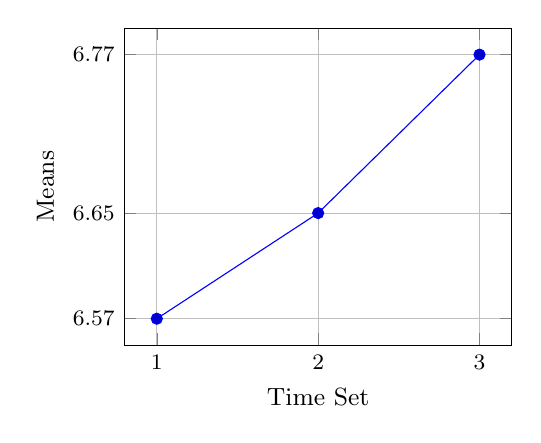
\begin{tikzpicture}
		\begin{axis}[xlabel = Time Set,ylabel = Means,small,xtick = {1,2,3}, ytick=data, grid=both]
		\addplot coordinates{(1,6.57) (2,6.65) (3,6.77)};
		\end{axis}
	\end{tikzpicture}
	\label{fig:ANOVApH1}
          \end{figure}
      \end{minipage}
      \hspace{0.05\linewidth}
      \begin{minipage}{0.45\linewidth}
          \begin{figure}[H]\centering
		\caption{pH set means, class 2}
 		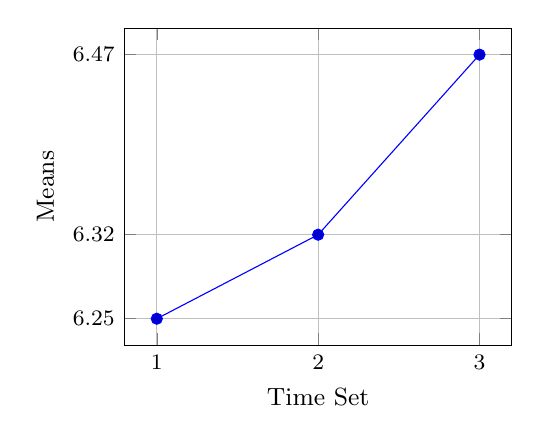
\begin{tikzpicture}
		\begin{axis}[xlabel = Time Set,ylabel = Means,small,xtick = {1,2,3}, ytick=data, grid=both]
		\addplot coordinates{(1,6.25) (2,6.32) (3,6.47)};
		\end{axis}
	\end{tikzpicture}
	\label{fig:ANOVApH2}
          \end{figure}
      \end{minipage}
   \hspace{0.05\linewidth}
      \begin{minipage}{0.45\linewidth}
          \begin{figure}[H]\centering
	\caption{pH set means, class 3}
        	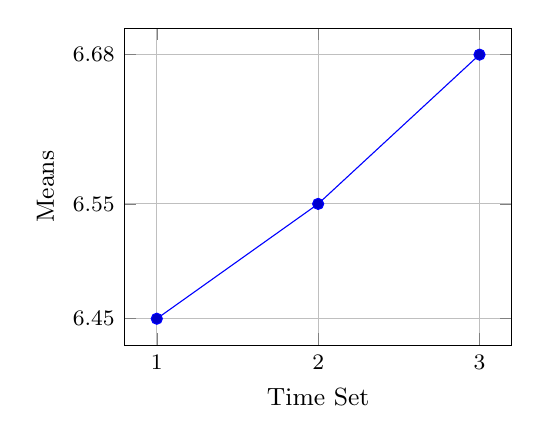
\begin{tikzpicture}	
		\begin{axis}[xlabel = Time Set,ylabel =Means,small,xtick = {1,2,3}, ytick=data, grid=both]
		\addplot coordinates{(1,6.45) (2,6.55) (3,6.68)};
		\end{axis}
	\end{tikzpicture}
	\label{fig:ANOVApH3}
          \end{figure}
      \end{minipage}
   \hspace{0.05\linewidth}
      \begin{minipage}{0.45\linewidth}
          \begin{figure}[H]\centering
	\caption{pH set means, class 4}
        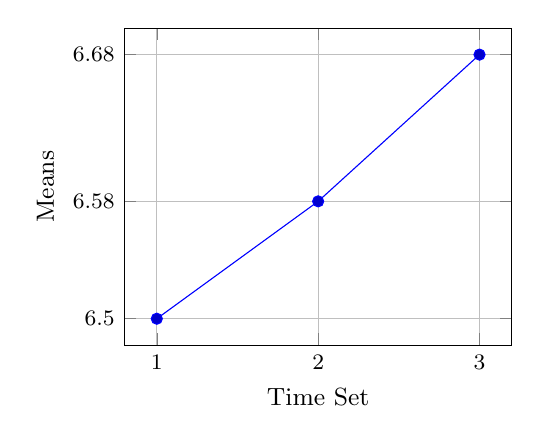
\begin{tikzpicture}
		\begin{axis}[xlabel = Time Set,ylabel = Means,small,xtick = {1,2,3}, ytick=data, grid=both]
		\addplot coordinates{(1,6.50) (2,6.58) (3,6.68)};
		\end{axis}
	\end{tikzpicture}
	\label{fig:ANOVApH4}
          \end{figure}
      \end{minipage}
   \hspace{0.05\linewidth}
      \begin{minipage}{0.45\linewidth}
          \begin{figure}[H]\centering
	\caption{pH set means, class 5}
        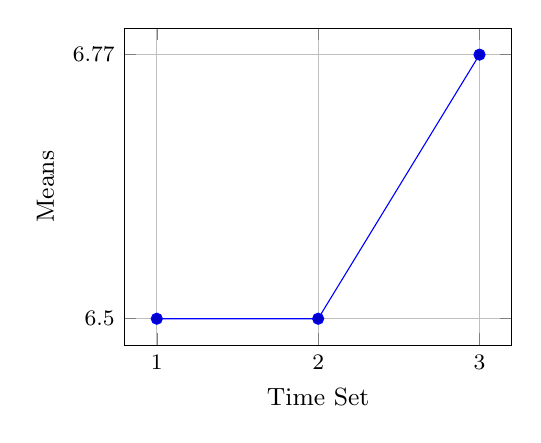
\begin{tikzpicture}
		\begin{axis}[xlabel = Time Set,ylabel =Means,small,xtick = {1,2,3}, ytick=data, grid=both]
		\addplot coordinates{(1,6.50) (2,6.50) (3,6.77)};
		\end{axis}
	\end{tikzpicture}
	\label{fig:ANOVApH5}
          \end{figure}
      \end{minipage}
   \hspace{0.05\linewidth}
      \begin{minipage}{0.45\linewidth}
          \begin{figure}[H]\centering
	\caption{pH set means, class 6}
        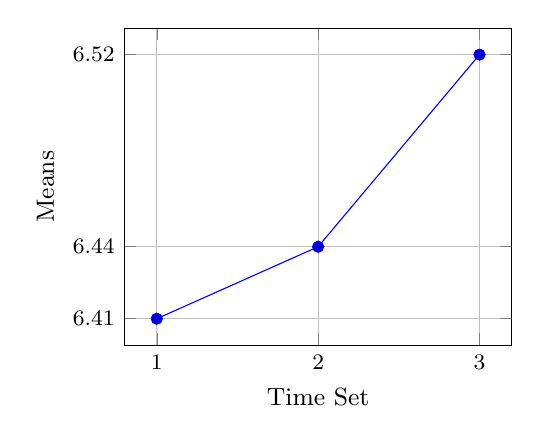
\begin{tikzpicture}	
		\begin{axis}[xlabel = Time Set,ylabel =Means,small,xtick = {1,2,3}, ytick=data, grid=both]
		\addplot coordinates{(1,6.41) (2,6.44) (3,6.52)};
		\end{axis}
	\end{tikzpicture}
	\label{fig:ANOVApH6}
          \end{figure}
      \end{minipage}
  \end{minipage}
  
%  \newpage
%\section{Figures}
%\subsection{Single figures}
%For more information, check: \href{http://en.wikibooks.org/wiki/LaTeX/Floats,_Figures_and_Captions}{http://en.wikibooks.org/wiki/LaTeX/Floats,\_Figures\_and\_Captions}
%\begin{verbatim}
    %\begin{figure}[t for top, b for bottom, h for here, ! to force placement]
        % Requires \usepackage{graphicx}
        %\centering % center the figure
        %\includegraphics[width=5in or 127mm etc...]{figure-name}\\
        %\caption{figure caption}\label{figure label}
    %\end{figure}
%\end{verbatim}
%\begin{figure}[h!]
  % Requires \usepackage{graphicx}
  %\centering
  %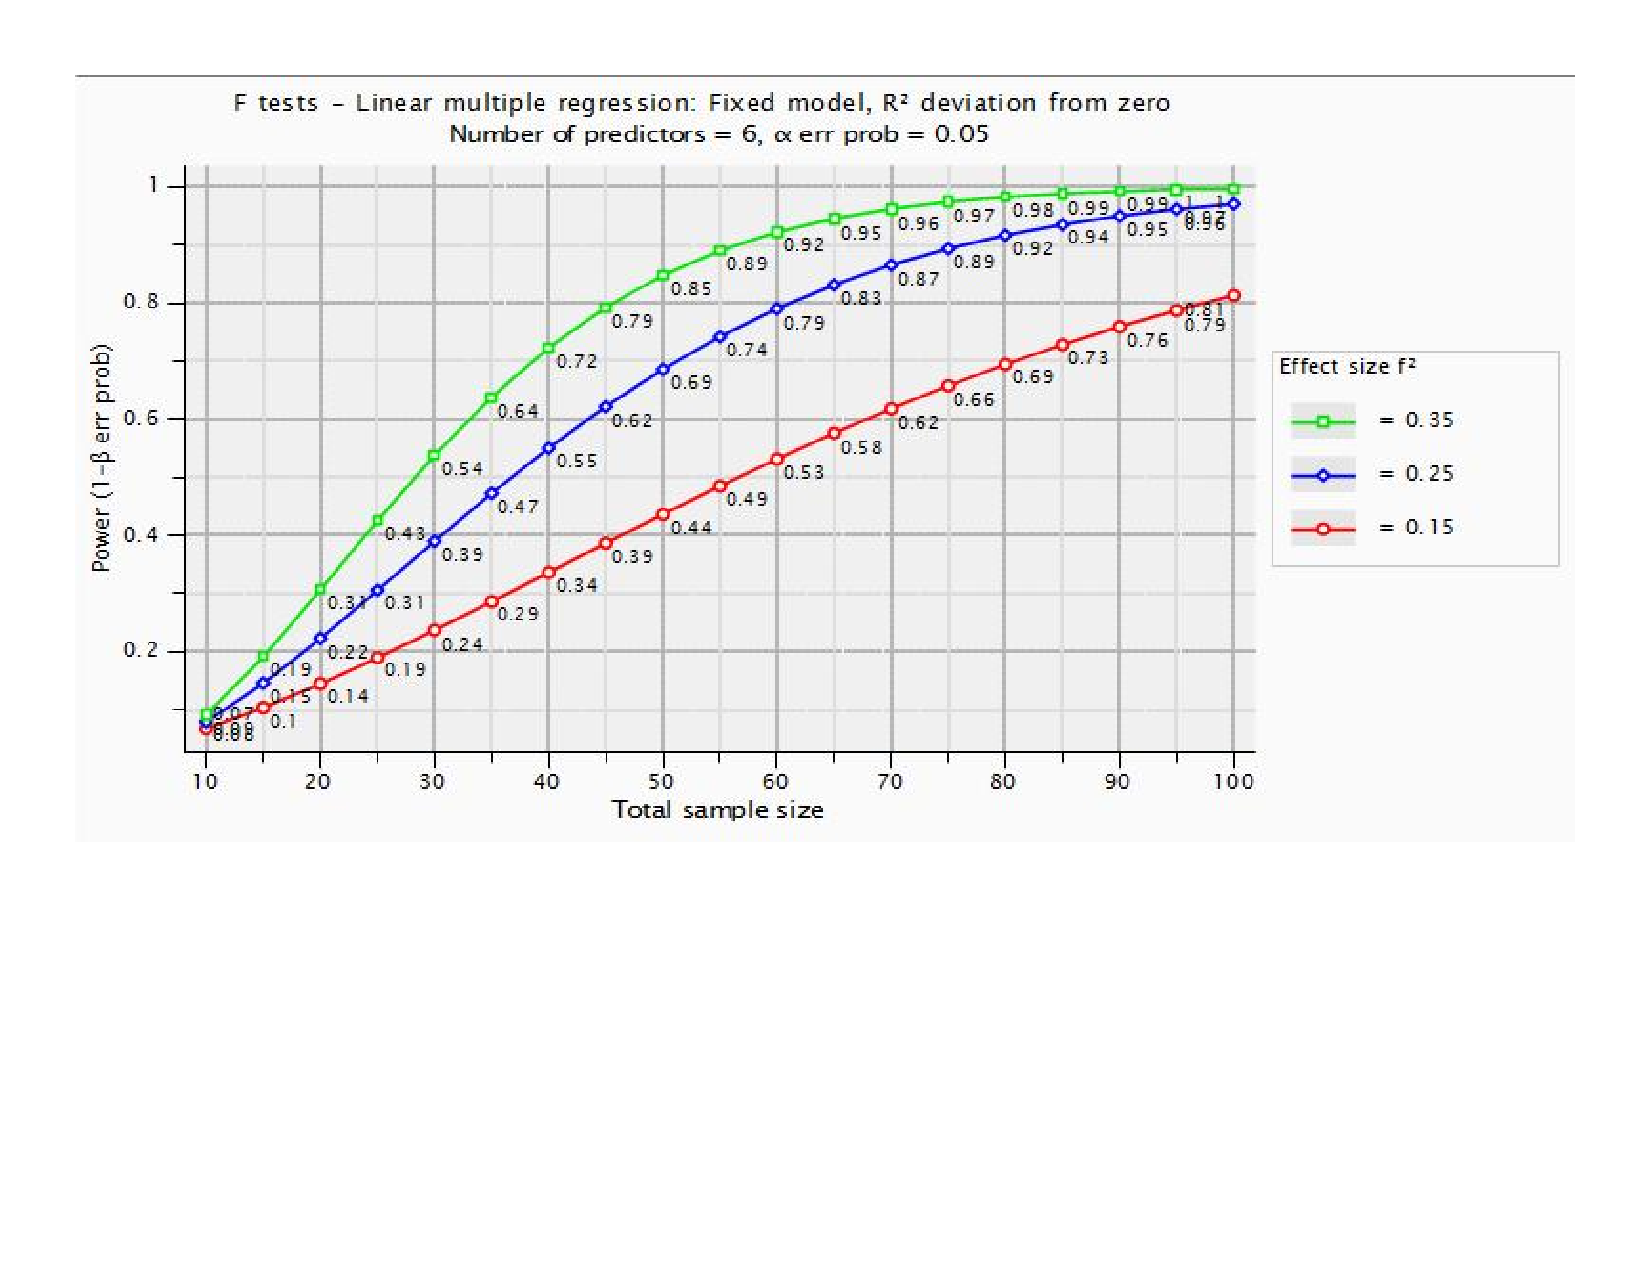
\includegraphics[width=3in]{pH}\\
  %\caption{Sample caption.}\label{label}
%\end{figure}
%\newpage
%\subsection{Multipart figures}
%For multipart figures, you need to use the package "subfig". here's an example
%\begin{verbatim}
%\begin{figure}
    %\centering
    %\subfloat[figure a]{\label{fig:figure-a} \includegraphics[width=w]{fig02a}}
    %\subfloat[figure b]{\label{fig:figure-b} \includegraphics[width=w]{fig02b}}
	%\subfloat[figure d]{\label{fig:figure-d} 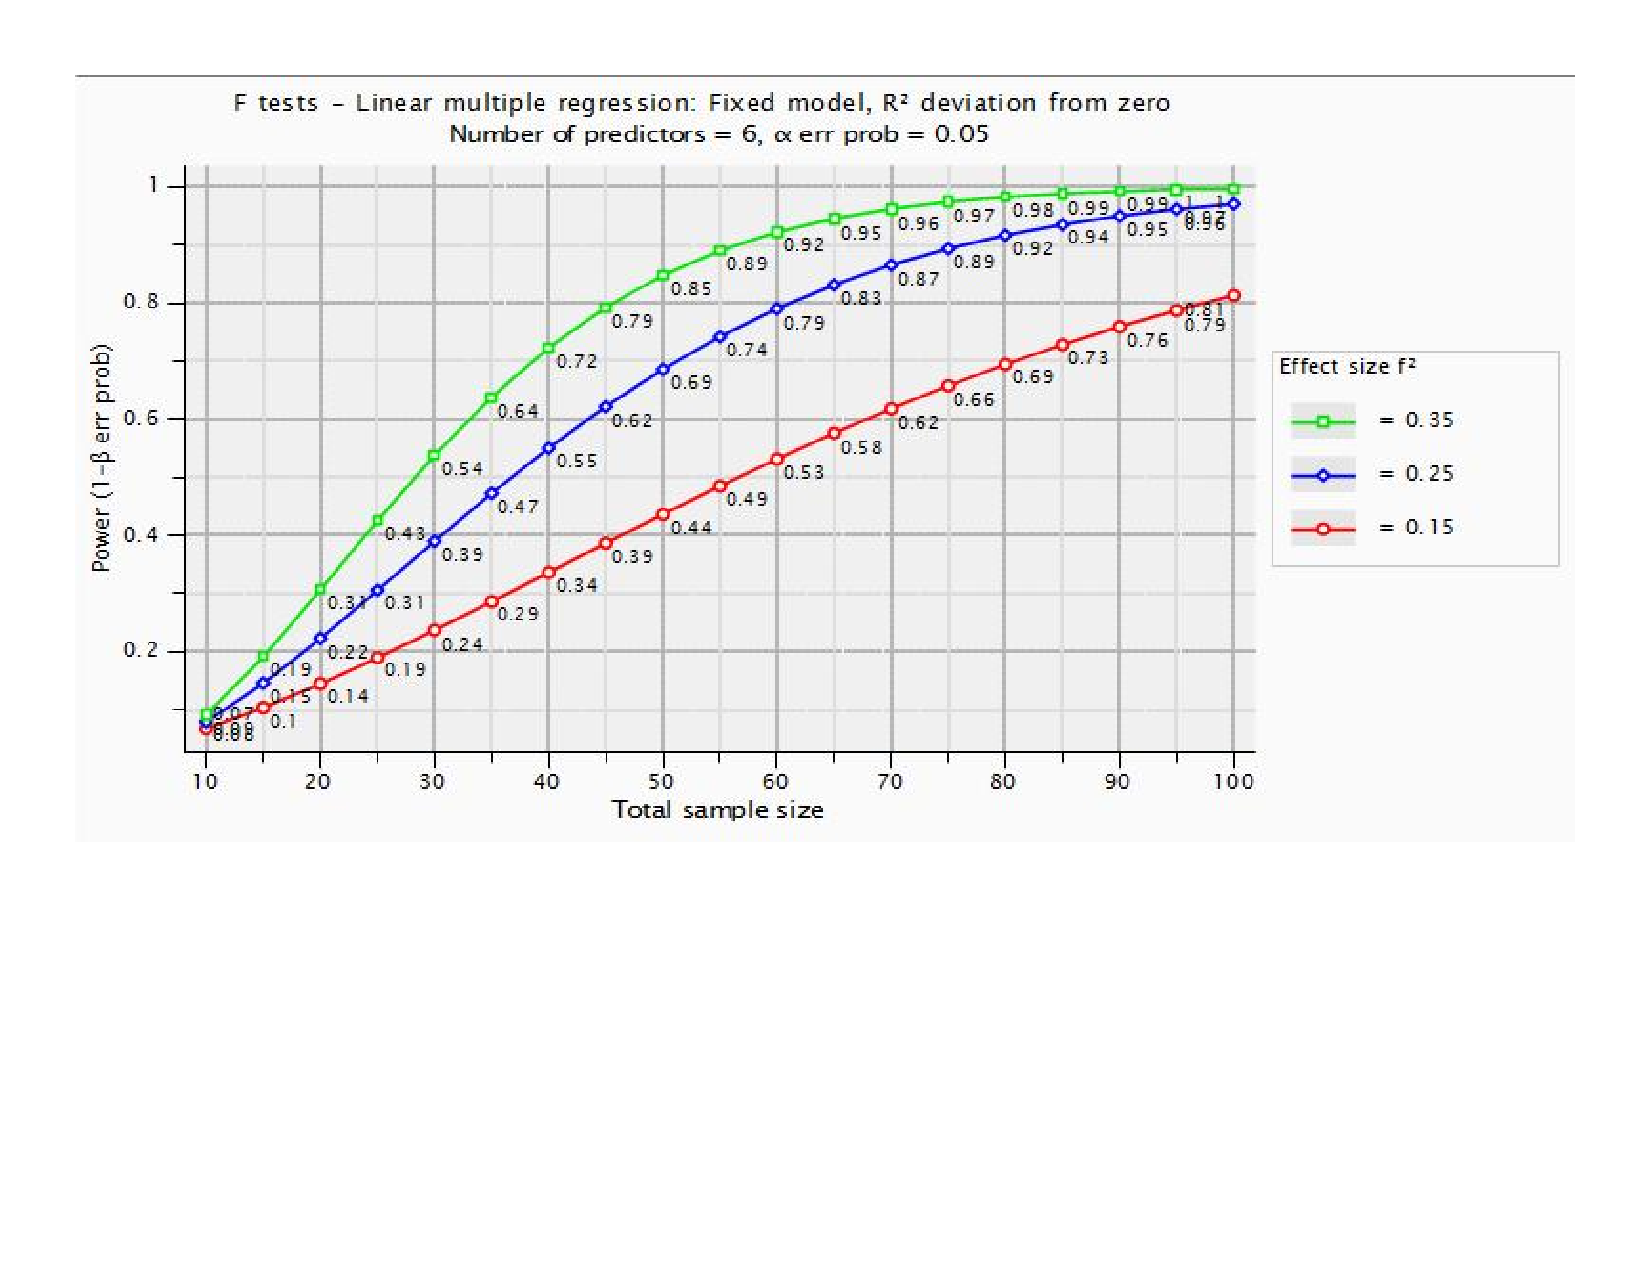
\includegraphics[width=w]{pH}}
    %\caption{Sample of a multipart figure} \label{fig:multipart-figure}
%\end{figure}
%\end{verbatim}
%\begin{figure}[h!]
    %    \centering
        %\subfloat[Circle]{\label{fig:figure-a}
\includegraphics[width=1.1in]{fig02a-circle}}
        %\subfloat[Rectangle]{\label{fig:figure-b}
\includegraphics[width=1.1in]{fig02b-rectangle}}
        %\subfloat[Cube]{\label{fig:figure-c}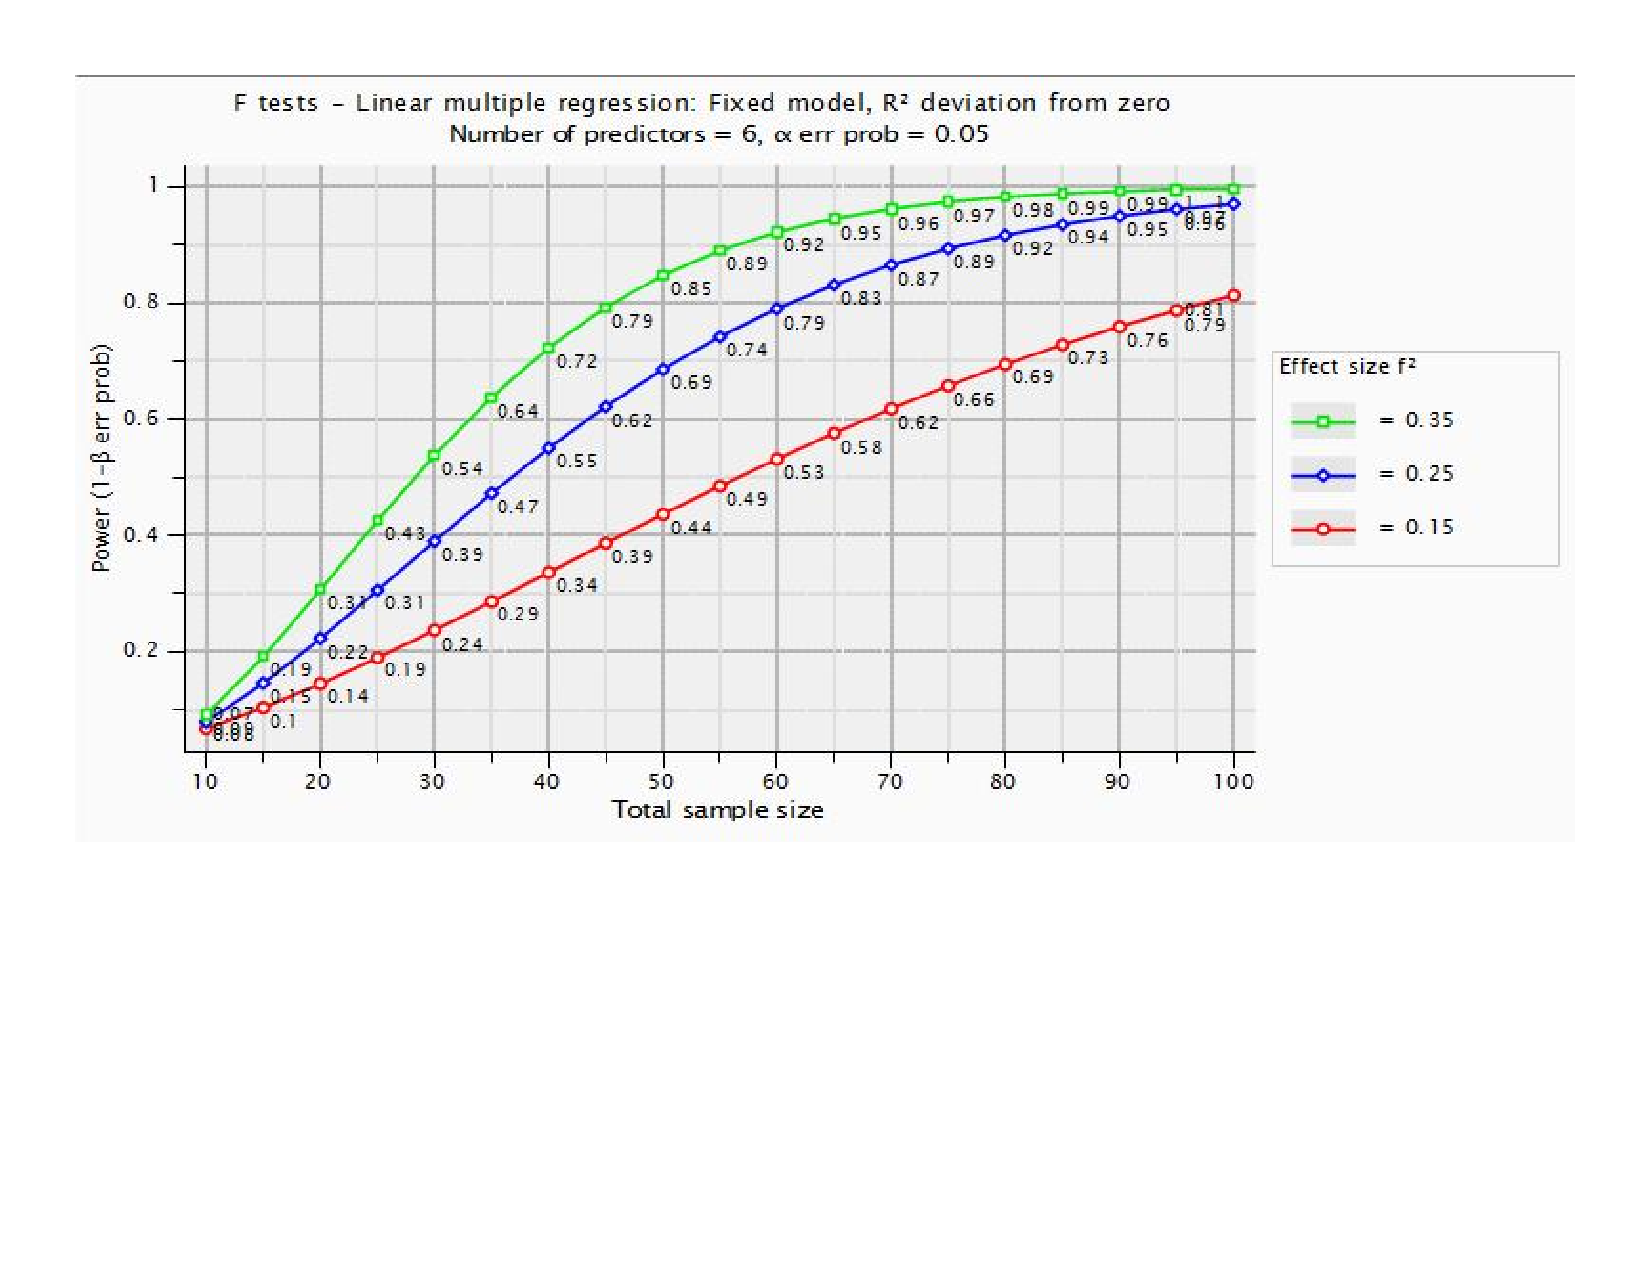
\includegraphics[width=1.1in]{pH}}
        %\caption{Geometric shapes.}
        %\label{fig:multipart-figure}
%\end{figure}
%To add some space between the figures above, one can use the usual spacing commands such as ``qquad''
%\begin{figure}[h!]
    %    \centering
        %\subfloat[Circle]{\label{fig:figure-a}
\includegraphics[width=1.1in]{fig02a-circle}} \qquad
        %\subfloat[Rectangle]{\label{fig:figure-b}
\includegraphics[width=1.1in]{fig02b-rectangle}}\qquad
        %\subfloat[Cube]{\label{fig:figure-c}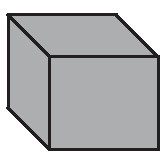
\includegraphics[width=1.1in]{fig02c-cube}}\qquad
        %\caption{Geometric shapes.}
        %\label{fig:multipart-figure}
%\end{figure} 
 
	\section{ANC}%decreasing ANC trends in Bonferoni
		  \begin{minipage}{\linewidth}
      \begin{minipage}{0.45\linewidth}
          \begin{figure}[H]
		\caption{ANC set means, class 1}
           	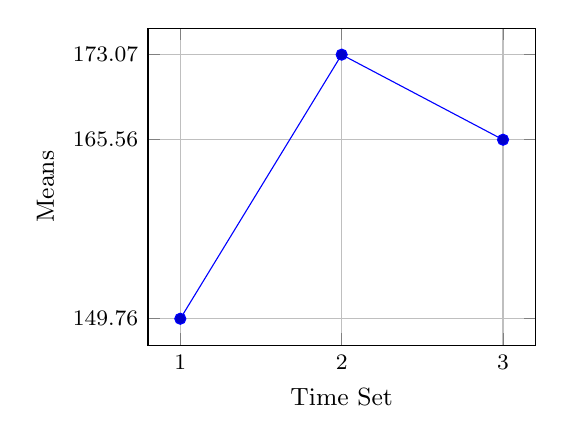
\begin{tikzpicture}
		\begin{axis}[xlabel = Time Set,ylabel = Means,small,xtick = {1,2,3}, ytick=data, grid=both]
		\addplot coordinates{(1,149.76) (2,173.07) (3,165.56)};
		\end{axis}
	\end{tikzpicture}
	\label{fig:ANOVAANC1}
          \end{figure}
      \end{minipage}
      \hspace{0.05\linewidth}
      \begin{minipage}{0.45\linewidth}
          \begin{figure}[H]
		\caption{ANC set means, class 2}
 		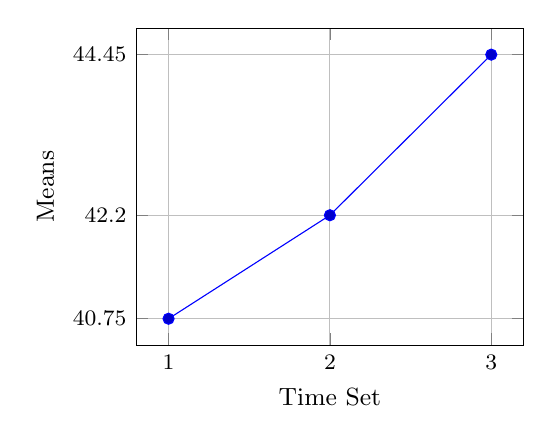
\begin{tikzpicture}
		\begin{axis}[xlabel = Time Set,ylabel = Means,small,xtick = {1,2,3}, ytick=data, grid=both]
		\addplot coordinates{(1,40.75) (2,42.20) (3,44.45)};
		\end{axis}
	\end{tikzpicture}
	\label{fig:ANOVAANC2}
          \end{figure}
      \end{minipage}
   \hspace{0.05\linewidth}
      \begin{minipage}{0.45\linewidth}
          \begin{figure}[H]
	\caption{ANC set means, class 3}
        	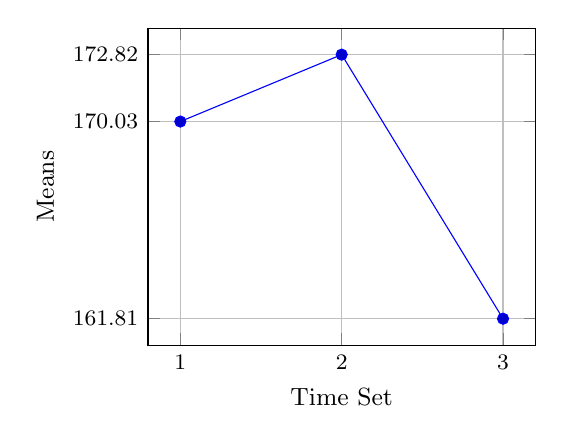
\begin{tikzpicture}
		\begin{axis}[xlabel = Time Set,ylabel =Means,small,xtick = {1,2,3}, ytick=data, grid=both]
		\addplot coordinates{(1,170.03) (2,172.82) (3,161.81)};
		\end{axis}
	\end{tikzpicture}
	\label{fig:ANOVAANC3}
          \end{figure}
      \end{minipage}
   \hspace{0.05\linewidth}
      \begin{minipage}{0.45\linewidth}
          \begin{figure}[H]
	\caption{ANC set means, class 4}
        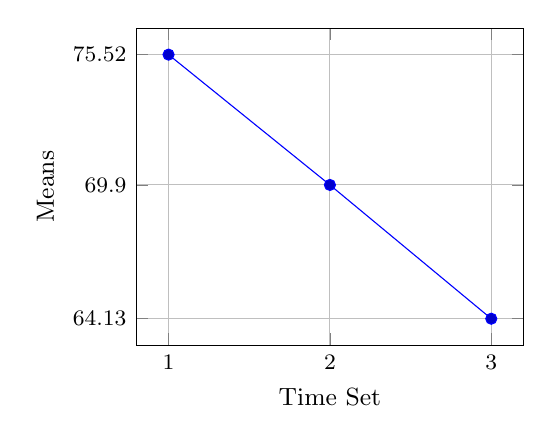
\begin{tikzpicture}
		\begin{axis}[xlabel = Time Set,ylabel = Means,small,xtick = {1,2,3}, ytick=data, grid=both]
		\addplot coordinates{(1,75.52) (2,69.90) (3,64.13)};
		\end{axis}
	\end{tikzpicture}
	\label{fig:ANOVAANC4}
          \end{figure}
      \end{minipage}
   \hspace{0.05\linewidth}
      \begin{minipage}{0.45\linewidth}
          \begin{figure}[H]
	\caption{ANC set means, class 5}
        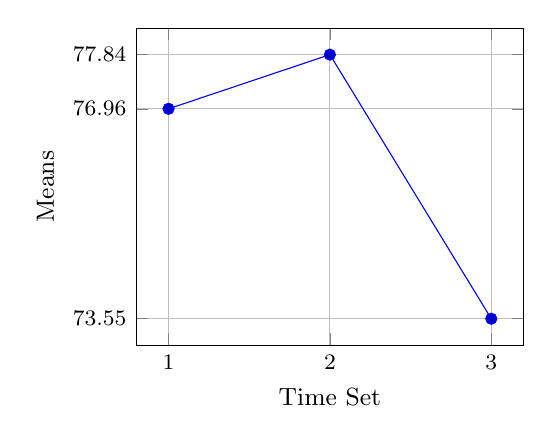
\begin{tikzpicture}
		\begin{axis}[xlabel = Time Set,ylabel =Means,small,xtick = {1,2,3}, ytick=data, grid=both]
		\addplot coordinates{(1,76.96) (2,77.84) (3,73.55)};
		\end{axis}
	\end{tikzpicture}
	\label{fig:ANOVAANC5}
          \end{figure}
      \end{minipage}
   \hspace{0.05\linewidth}
      \begin{minipage}{0.45\linewidth}
          \begin{figure}[H]
	\caption{ANC set means, class 6}
        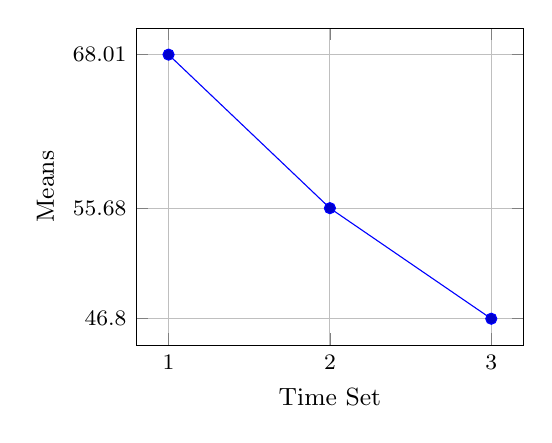
\begin{tikzpicture}
		\begin{axis}[xlabel = Time Set,ylabel =Means,small,xtick = {1,2,3}, ytick=data, grid=both]
		\addplot coordinates{(1,68.01) (2,55.68) (3,46.80)};
		\end{axis}
	\end{tikzpicture}
	\label{fig:ANOVAANC6}
          \end{figure}
      \end{minipage}
  \end{minipage}

	\section{Nitrate}
		  \begin{minipage}{\linewidth}
      \begin{minipage}{0.45\linewidth}
          \begin{figure}[H]
           	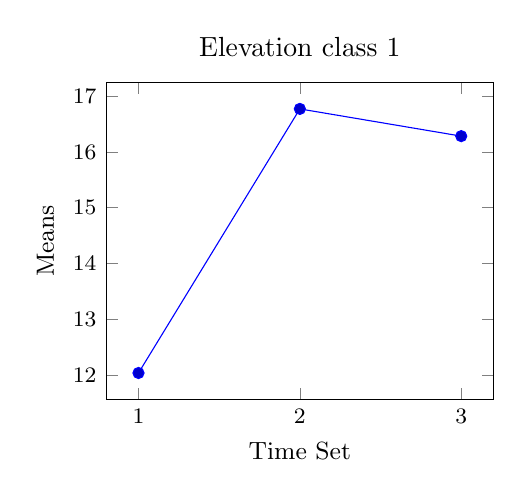
\begin{tikzpicture}
		\begin{axis}[title=Elevation class 1, xlabel = Time Set,ylabel = Means,small,xtick = {1,2,3}]
		\addplot coordinates{(1,12.03733) (2,16.77264) (3,16.28445)};
		\end{axis}
	\end{tikzpicture}
	\label{fig:ANOVANO31}
          \end{figure}
      \end{minipage}
      \hspace{0.05\linewidth}
      \begin{minipage}{0.45\linewidth}
          \begin{figure}[H]
 		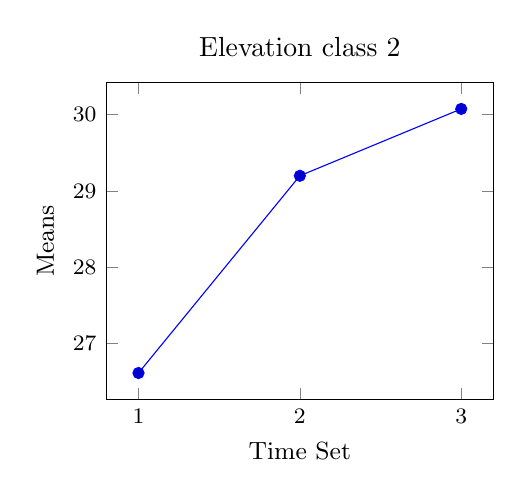
\begin{tikzpicture}
		\begin{axis}[title=Elevation class 2 , xlabel = Time Set,ylabel = Means,small,xtick = {1,2,3}]
		\addplot coordinates{(1,26.61657) (2,29.20006) (3,30.07626)};
		\end{axis}
	\end{tikzpicture}
	\label{fig:ANOVANO32}
          \end{figure}
      \end{minipage}
   \hspace{0.05\linewidth}
      \begin{minipage}{0.45\linewidth}
          \begin{figure}[H]
        	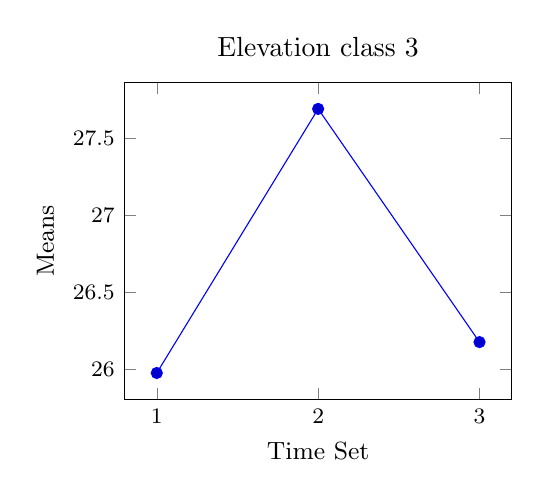
\begin{tikzpicture}
		\begin{axis}[title=Elevation class 3,xlabel = Time Set,ylabel =Means,small,xtick = {1,2,3}]
		\addplot coordinates{(1,25.97658) (2,27.68893) (3,26.17686)};
		\end{axis}
	\end{tikzpicture}
	\label{fig:ANOVANO33}
          \end{figure}
      \end{minipage}
   \hspace{0.05\linewidth}
      \begin{minipage}{0.45\linewidth}
          \begin{figure}[H]
        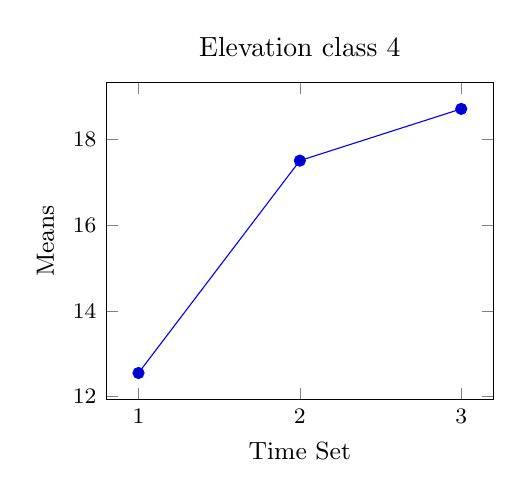
\begin{tikzpicture}
		\begin{axis}[title=Elevation class 4,xlabel = Time Set,ylabel = Means,small,xtick = {1,2,3}]
		\addplot coordinates{(1,12.55250) (2,17.50807) (3,18.71509)};
		\end{axis}
	\end{tikzpicture}
	\label{fig:ANOVANO34}
          \end{figure}
      \end{minipage}
   \hspace{0.05\linewidth}
      \begin{minipage}{0.45\linewidth}
          \begin{figure}[H]
        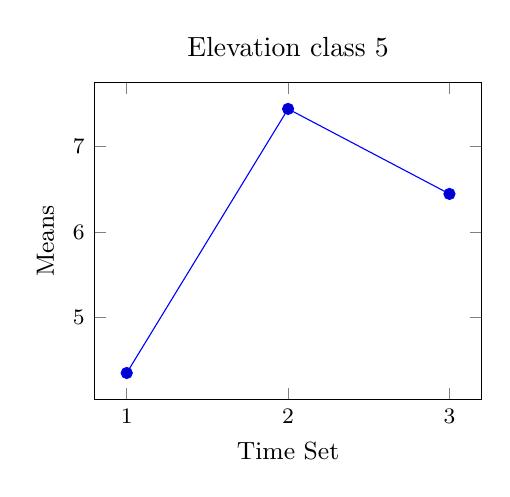
\begin{tikzpicture}
		\begin{axis}[title=Elevation class 5,xlabel = Time Set,ylabel =Means,small,xtick = {1,2,3}]
		\addplot coordinates{(1,4.35218) (2,7.43691) (3,6.44408)};
		\end{axis}
	\end{tikzpicture}
	\label{fig:ANOVANO35}
          \end{figure}
      \end{minipage}
   \hspace{0.05\linewidth}
      \begin{minipage}{0.45\linewidth}
          \begin{figure}[H]
        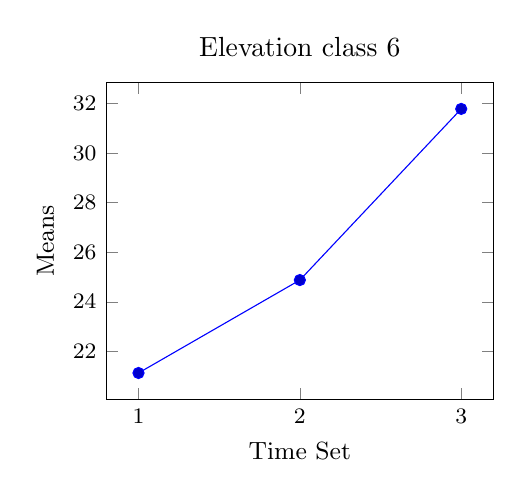
\begin{tikzpicture}
		\begin{axis}[title=Elevation class 6,xlabel = Time Set,ylabel =Means,small,xtick = {1,2,3}]
		\addplot coordinates{(1,21.13072) (2,24.87664) (3,31.77411)};
		\end{axis}
	\end{tikzpicture}
	\label{fig:ANOVANO36}
          \end{figure}
      \end{minipage}
  \end{minipage}

	\section{Sulfate}
		  \begin{minipage}{\linewidth}
      \begin{minipage}{0.45\linewidth}
          \begin{figure}[H]
           	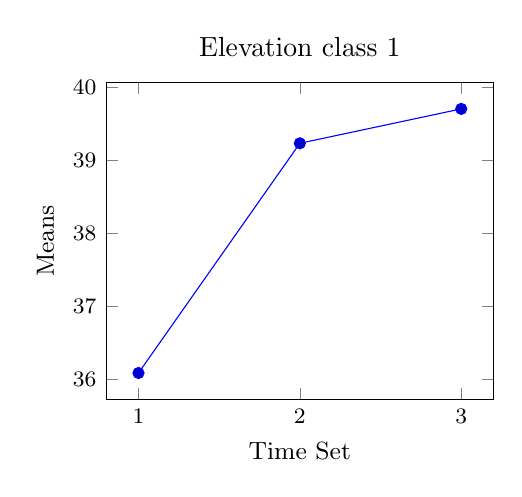
\begin{tikzpicture}
		\begin{axis}[title=Elevation class 1, xlabel = Time Set,ylabel = Means,small,xtick = {1,2,3}]
		\addplot coordinates{(1,36.09) (2,39.23) (3,39.70)};
		\end{axis}
	\end{tikzpicture}
	\label{fig:ANOVASO41}
          \end{figure}
      \end{minipage}
      \hspace{0.05\linewidth}
      \begin{minipage}{0.45\linewidth}
          \begin{figure}[H]
 		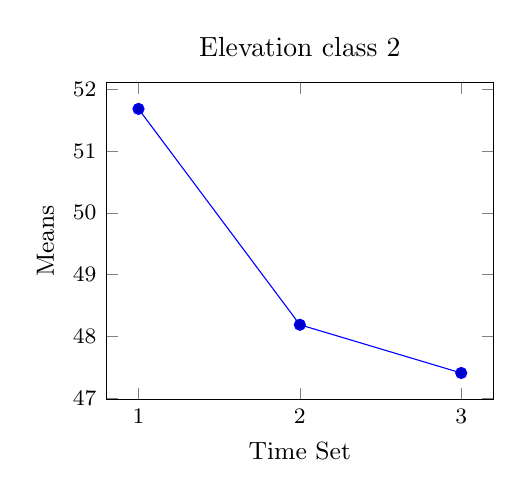
\begin{tikzpicture}
		\begin{axis}[title=Elevation class 2 , xlabel = Time Set,ylabel = Means,small,xtick = {1,2,3}]
		\addplot coordinates{(1,51.68) (2,48.19) (3,47.41)};
		\end{axis}
	\end{tikzpicture}
	\label{fig:ANOVASO42}
          \end{figure}
      \end{minipage}
   \hspace{0.05\linewidth}
      \begin{minipage}{0.45\linewidth}
          \begin{figure}[H]
        	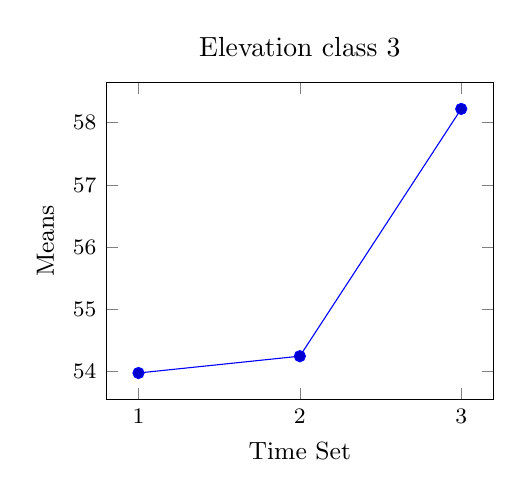
\begin{tikzpicture}
		\begin{axis}[title=Elevation class 3,xlabel = Time Set,ylabel =Means,small,xtick = {1,2,3}]
		\addplot coordinates{(1,53.98) (2,54.25) (3,58.22)};
		\end{axis}
	\end{tikzpicture}
	\label{fig:ANOVASO43}
          \end{figure}
      \end{minipage}
   \hspace{0.05\linewidth}
      \begin{minipage}{0.45\linewidth}
          \begin{figure}[H]
        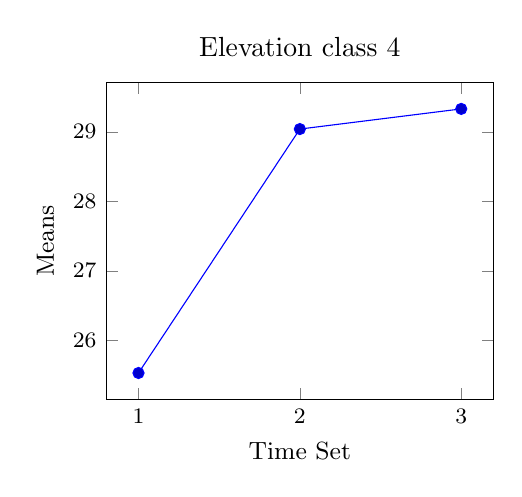
\begin{tikzpicture}
		\begin{axis}[title=Elevation class 4,xlabel = Time Set,ylabel = Means,small,xtick = {1,2,3}]
		\addplot coordinates{(1,25.53) (2,29.04) (3,29.33)};
		\end{axis}
	\end{tikzpicture}
	\label{fig:ANOVASO44}
          \end{figure}
      \end{minipage}
   \hspace{0.05\linewidth}
      \begin{minipage}{0.45\linewidth}
          \begin{figure}[H]
        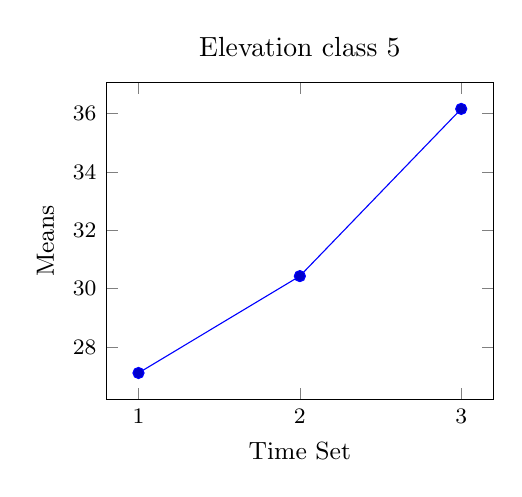
\begin{tikzpicture}
		\begin{axis}[title=Elevation class 5,xlabel = Time Set,ylabel =Means,small,xtick = {1,2,3}]
		\addplot coordinates{(1,27.11) (2,30.43) (3,36.16)};
		\end{axis}
	\end{tikzpicture}
	\label{fig:ANOVASO45}
          \end{figure}
      \end{minipage}
   \hspace{0.05\linewidth}
      \begin{minipage}{0.45\linewidth}
          \begin{figure}[H]
        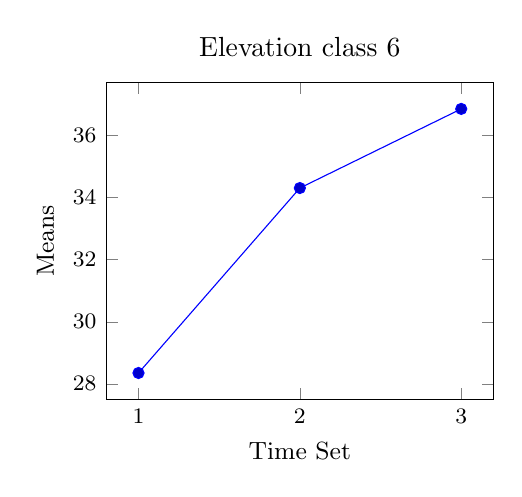
\begin{tikzpicture}
		\begin{axis}[title=Elevation class 6,xlabel = Time Set,ylabel =Means,small,xtick = {1,2,3}]
		\addplot coordinates{(1,28.35) (2,34.31) (3,36.86)};
		\end{axis}
	\end{tikzpicture}
	\label{fig:ANOVASO46}
          \end{figure}
      \end{minipage}
  \end{minipage}


\chapter{Post Hoc Power Analsysis}
	\section{Step-Wise Variables}
		%\begin{landscape}\footnotesize
\begin{sidewaystable}[p]\footnotesize
\caption{Post hoc power analysis using G*power and a calculated ES, $\alpha$ is .05.\textbf{Bold} results are insignificant.}
\begin{tabular}{p{1cm}p{.5cm}cccccccccccccccc}
\hline\noalign{\smallskip}
\multicolumn{1}{c}{}&\multicolumn{1}{c}{}  & \multicolumn{4}{c}{pH} &\multicolumn{4}{c}{ ANC $\mu$eqL} & \multicolumn{4}{c}{ Nitrate $\mu$eqL} &  \multicolumn{4}{c}{Sulfate $\mu$eqL}  \\ \cline{3-18}\noalign{\smallskip}
 & \multicolumn{ 1}{c}{} & \multicolumn{ 1}{c}{} &  \\ 
 \multicolumn{ 1}{c}{Set} & \multicolumn{ 1}{c}{Class} & \multicolumn{ 1}{c}{N} & \multicolumn{ 1}{p{1.2cm}}{Adjusted r$^2$} & \multicolumn{ 1}{p{1cm}}{Effect Size} & \multicolumn{ 1}{p{1cm}}{Actual Power} & \multicolumn{ 1}{c}{N} & \multicolumn{ 1}{p{1.2cm}}{Adjusted r$^2$} & \multicolumn{ 1}{p{1cm}}{Effect Size} & \multicolumn{ 1}{p{1cm}}{Actual Power} & \multicolumn{ 1}{c}{N} & \multicolumn{ 1}{p{1.2cm}}{Adjusted r$^2$} & \multicolumn{ 1}{p{1cm}}{Effect Size} & \multicolumn{ 1}{p{1cm}}{Actual Power} & \multicolumn{ 1}{c}{N} & \multicolumn{ 1}{p{1.2cm}}{Adjusted r$^2$} & \multicolumn{ 1}{p{1cm}}{Effect Size}& \multicolumn{1}{p{1cm}}{Actual Power} \\ \hline\noalign{\smallskip}
1993-2002\\
 & \multicolumn{1}{c}{1} & 327 & \multicolumn{ 1}{c}{0.712} & \multicolumn{ 1}{c}{2.47} & \multicolumn{ 1}{c}{1.00} & \multicolumn{ 1}{c}{327} & \multicolumn{ 1}{c}{0.985} & \multicolumn{ 1}{c}{65.67} & \multicolumn{ 1}{c}{1.00} & \multicolumn{ 1}{c}{275} & \multicolumn{ 1}{c}{0.503} & \multicolumn{ 1}{c}{1.01} & \multicolumn{ 1}{c}{1.00} & \multicolumn{ 1}{c}{325} & \multicolumn{ 1}{c}{0.569} & \multicolumn{ 1}{c}{1.32} & \multicolumn{ 1}{c}{1.00} \\ 
 & \multicolumn{ 1}{c}{2} & 393 & 0.388  & 0.63  & 1.00  & 392 & 0.603  & 1.52  & 1.00  & 377 & 0.699  & 2.32  & 1.00  & 390 & 0.766  & 3.27  & 1.00  \\ 
 & \multicolumn{ 1}{c}{3} & 400 & 0.693  & 2.26  & 1.00  & 398 & 0.971  & 33.48  & 1.00  & 365 & 0.359  & 0.56  & 1.00  & 391 & 0.590  & 1.44  & 1.00  \\ 
 & \multicolumn{ 1}{c}{4} & 121 & 0.205  & 0.26  & 0.99  & 120 & 0.709  & 2.44  & 1.00  & 105 & 0.410  & 0.69  & 1.00  & 119 & 0.402  & 0.67  & 1.00  \\ 
 & \multicolumn{ 1}{c}{5} & 116 & 0.165  & 0.20  & 0.96  & 116 & 0.760  & 3.17  & 1.00  & 66 & 0.328  & 0.49  & 0.98  & 116 & 0.566  & 1.30  & 1.00  \\ 
 & \multicolumn{ 1}{c}{6} & 110 & 0.505 & 1.02  & 1.00  & 110 & 0.802 & 4.05  & 1.00  & 81 & 0.871  & 6.75  & 1.00  & 110 & 0.716  & 2.52  & 1.00  \\ 
2003-2008\\
 & \multicolumn{ 1}{c}{1} & 255 & 0.781  & 3.57  & 1.00  & 255 & 0.996  & 249.00  & 1.00  & 252 & 0.551  & 1.23  & 1.00  & 261 & 0.673  & 2.06  & 1.00  \\ 
 & \multicolumn{ 1}{c}{2} & 289 & 0.348  & 0.53  & 1.00  & 289 & 0.779  & 3.52  & 1.00  & 296 & 0.816  & 4.43  & 1.00  & 298 & 0.893  & 8.35  & 1.00  \\ 
 & \multicolumn{ 1}{c}{3} & 299 & 0.663  & 1.97  & 1.00  & 299 & 0.996  & 249.00  & 1.00  & 297 & 0.637  & 1.75  & 1.00  & 308 & 0.923  & 11.99  & 1.00  \\ 
 & \multicolumn{ 1}{c}{4} & 119 & 0.400  & 0.67  & 1.00  & 119 & 0.779  & 3.52  & 1.00  & 121 & 0.405  & 0.68  & 1.00  & 123 & 0.343  & 0.52  & 1.00  \\ 
 & \multicolumn{ 1}{c}{5} & 35 & 0.300  & 0.43  & 0.74  & 35 & 0.739  & 2.83  & 1.00  & 30 & 0.562  & 1.28  & 0.98  & 37 & 0.884  & 7.62  & 1.00  \\ 
 & \multicolumn{ 1}{c}{6} & 97 & 0.317 & 0.46  & 1.00  & 97 & 0.812 & 4.32  & 1.00  & 98 & 0.832  & 4.95  & 1.00  & 101 & 0.844  & 5.41  & 1.00  \\ 
2009-2012\\
 & \multicolumn{ 1}{c}{1} & 191 & 0.894  & 8.43  & 1.00  & 191 & 0.989  & 89.91  & 1.00  & 191 & 0.376  & 0.60  & 1.00  & 190 & 0.536  & 1.16  & 1.00  \\ 
\multicolumn{ 1}{c}{} & \multicolumn{ 1}{c}{2} & 212 & 0.606  & 1.54  & 1.00  & 212 & 0.862  & 6.25  & 1.00  & 212 & 0.735  & 2.77  & 1.00  & 212 & 0.887  & 7.85  & 1.00  \\ 
\multicolumn{ 1}{c}{} & \multicolumn{ 1}{c}{3} & 228 & 0.766  & 3.27  & 1.00  & 228 & 0.997  & 332.33  & 1.00  & 228 & 0.598  & 1.49  & 1.00  & 228 & 0.915  & 10.76  & 1.00  \\ 
\multicolumn{ 1}{c}{} & \multicolumn{ 1}{c}{4} & 97 & 0.593  & 1.46  & 1.00  & 97 & 0.772  & 3.39  & 1.00  & 97 & 0.635  & 1.74  & 1.00  & 97 & 0.529  & 1.12  & 1.00  \\ 
\multicolumn{ 1}{c}{} & \multicolumn{ 1}{c}{5} & 29 & \textbf{0.158 } & 0.19  & 0.28  & 29 & 0.540  & 1.17  & 0.96  & 29 & \textbf{-0.272 } & NA & NA & 29 & 0.658  & 1.92  & 1.00  \\ 
\multicolumn{ 1}{c}{} & \multicolumn{ 1}{c}{6} & 76 & 0.286 & 0.40  & 0.99  & 76 & 0.809 & 4.24  & 1.00  & 76 & 0.881  & 7.40  & 1.00  & 76 & 0.861  & 6.19  & 1.00  \\ \hline
\end{tabular}
\label{tab:SWposthoc}
\end{sidewaystable}
%\end{landscape}
%needs cleaning


	\section{Temperol variables}
		\begin{sidewaystable}[p]\footnotesize
\caption{Post hoc power analysis using G*power a calculated ES, an alpha of .05 with the variables: $\sin(\theta)$, $\cos(\theta)$, and Julian date only.   \textbf{Bold} results are insignificant.}
\begin{tabular}{p{1cm}p{.5cm}cccccccccccccccc}
\hline\noalign{\smallskip}
\multicolumn{1}{c}{}&\multicolumn{1}{c}{}  & \multicolumn{4}{c}{pH} &\multicolumn{4}{c}{ ANC $\mu$eqL} & \multicolumn{4}{c}{ Nitrate $\mu$eqL} &  \multicolumn{4}{c}{Sulfate $\mu$eqL}  \\ \cline{3-18}\noalign{\smallskip}
 & \multicolumn{ 1}{c}{} & \multicolumn{ 1}{c}{} &  \\ 
 \multicolumn{ 1}{c}{Set} & \multicolumn{ 1}{c}{Class} & \multicolumn{ 1}{c}{N} & \multicolumn{ 1}{p{1.2cm}}{Adjusted r$^2$} & \multicolumn{ 1}{p{1cm}}{Effect Size} & \multicolumn{ 1}{p{1cm}}{Actual Power} & \multicolumn{ 1}{c}{N} & \multicolumn{ 1}{p{1.2cm}}{Adjusted r$^2$} & \multicolumn{ 1}{p{1cm}}{Effect Size} & \multicolumn{ 1}{p{1cm}}{Actual Power} & \multicolumn{ 1}{c}{N} & \multicolumn{ 1}{p{1.2cm}}{Adjusted r$^2$} & \multicolumn{ 1}{p{1cm}}{Effect Size} & \multicolumn{ 1}{p{1cm}}{Actual Power} & \multicolumn{ 1}{c}{N} & \multicolumn{ 1}{p{1.2cm}}{Adjusted r$^2$} & \multicolumn{ 1}{p{1cm}}{Effect Size}& \multicolumn{1}{p{1cm}}{Actual Power} \\ \hline\noalign{\smallskip}
1993-2002\\
& \multicolumn{1}{c}{1} & 327 & \textbf{0.047} & 0.049 & 0.93 & 327 & \textbf{0.024} & 0.02 & 0.65 & 275 & 0.016 & 0.02 & 0.39 & 325 & 0.045 & 0.05 & 0.92 \\ 
 & \multicolumn{ 1}{c}{2} & 393 & \textbf{0.128 } & 0.15  & 1.00  & 392 & \textbf{0.189 } & 0.23  & 1.00  & 377 & \textbf{0.017 } & 0.02  & 0.55  & 390 & \textbf{0.009 } & 0.01  & 0.32  \\ 
 & \multicolumn{ 1}{c}{3} & 400 & \textbf{0.013 } & 0.01  & 0.46  & 398 & \textbf{0.000 } & 0.00  & 0.06  & 365 & \textbf{-0.004 } & NA & NA & 391 & \textbf{-0.004 } &  NA & NA \\ 
 & \multicolumn{ 1}{c}{4} & 121 & \textbf{0.059 } & 0.06  & 0.61  & 120 & \textbf{0.294 } & 0.42  & 1.00  & 105 & \textbf{-0.027 } & NA & NA & 119 & \textbf{-0.016 } & NA & NA \\ 
 & \multicolumn{ 1}{c}{5} & 116 & \textbf{0.051 } & 0.05  & 0.52  & 116 & 0.381  & 0.62  & 1.00  & 66 & 0.120  & 0.14  & 0.68  & 116 & \textbf{-0.010 } & NA & NA \\ 
 & \multicolumn{ 1}{c}{6} & 110 & \textbf{0.096 } & 0.11  & 0.81  & 110 & \textbf{0.075 } & 0.08  & 0.69  & 81 & \textbf{0.092 } & 0.10  & 0.64  & 110 & \textbf{-0.009 } & NA & NA \\ 
2003-2008 \\
& \multicolumn{ 1}{c}{1} & 255 & 0.040  & 0.04  & 0.78  & 255 & \textbf{0.001 } & 0.00  & 0.07  & 252 & 0.061  & 0.06  & 0.94  & 261 & 0.043  & 0.04  & 0.82  \\ 
 & \multicolumn{ 1}{c}{2} & 289 & 0.061  & 0.06  & 0.96  & 289 & \textbf{0.081 } & 0.09  & 0.99  & 296 & 0.043  & 0.04  & 0.87  & 298 & 0.014  & 0.01  & 0.37  \\ 
 & \multicolumn{ 1}{c}{3} & 299 & \textbf{0.020 } & 0.02  & 0.52  & 299 & \textbf{-0.003 } & NA & NA & 297 & \textbf{-0.003 } & NA & NA & 308 & \textbf{0.006 } & 0.01  & 0.18  \\ 
 & \multicolumn{ 1}{c}{4} & 119 & 0.148  & 0.17  & 0.97  & 119 & \textbf{0.180 } & 0.22  & 0.99  & 121 & 0.086  & 0.09  & 0.80  & 123 & 0.023  & 0.02  & 0.26  \\ 
 & \multicolumn{ 1}{c}{5} & 35 & \textbf{-0.069 } & NA & NA & 35 & \textbf{0.337 } & 0.51  & 0.93  & 30 & \textbf{-0.082 } & NA & NA & 37 & \textbf{-0.024 } & NA & NA \\ 
 & \multicolumn{ 1}{c}{6} & 97 & 0.081  & 0.09  & 0.67  & 97 & \textbf{0.094 } & 0.10  & 0.74  & 98 & 0.046  & 0.05  & 0.40  & 101 & 0.074  & 0.08  & 0.64  \\ 
2009-2012\\
 & \multicolumn{ 1}{c}{1} & 191 & \textbf{0.028 } & 0.03  & 0.47  & 191 & \textbf{0.000 } & 0.00  & 0.05  & 191 & \textbf{0.018 } & 0.02  & 0.31  & 190 & \textbf{0.005 } & 0.01  & 0.11  \\ 
\multicolumn{ 1}{c}{} & \multicolumn{ 1}{c}{2} & 212 & 0.052  & 0.05  & 0.82  & 212 & \textbf{0.056 } & 0.06  & 0.85  & 212 & \textbf{0.011 } & 0.01  & 0.22  & 212 & \textbf{-0.010 } & NA & NA \\ 
\multicolumn{ 1}{c}{} & \multicolumn{ 1}{c}{3} & 228 & \textbf{-0.009 } & NA & NA & 228 & \textbf{-0.002 } & NA & NA & 228 & \textbf{-0.004 } & NA & NA & 228 & \textbf{-0.007 } & NA & NA \\ 
\multicolumn{ 1}{c}{} & \multicolumn{ 1}{c}{4} & 97 & 0.200  & 0.25  & 0.99  & 97 & \textbf{0.161 } & 0.19  & 0.96  & 97 & \textbf{-0.016 } & NA & NA & 97 & \textbf{-0.011 } & NA & NA \\ 
\multicolumn{ 1}{c}{} & \multicolumn{ 1}{c}{5} & 29 & \textbf{0.218 } & 0.28  & 0.58  & 29 & 0.466  & 0.87  & 0.98  & 29 & \textbf{-0.039 } & NA & NA & 29 & \textbf{-0.076 } & NA & NA \\ 
\multicolumn{ 1}{c}{} & \multicolumn{ 1}{c}{6} & 76 & 0.039  & 0.04  & 0.27  & 76 & \textbf{0.058 } & 0.06  & 0.39  & 76 & \textbf{-0.016 } & NA & NA & 76 & \textbf{0.007 } & 0.01  & 0.08  \\ 
\end{tabular}
\label{tab:TVposthoc}
\end{sidewaystable}%needs cleaning


\chapter{A priori analysis}\label{ch:APA}
	\section{Power graphs}
		\subsection{pH}
			\begin{figure}
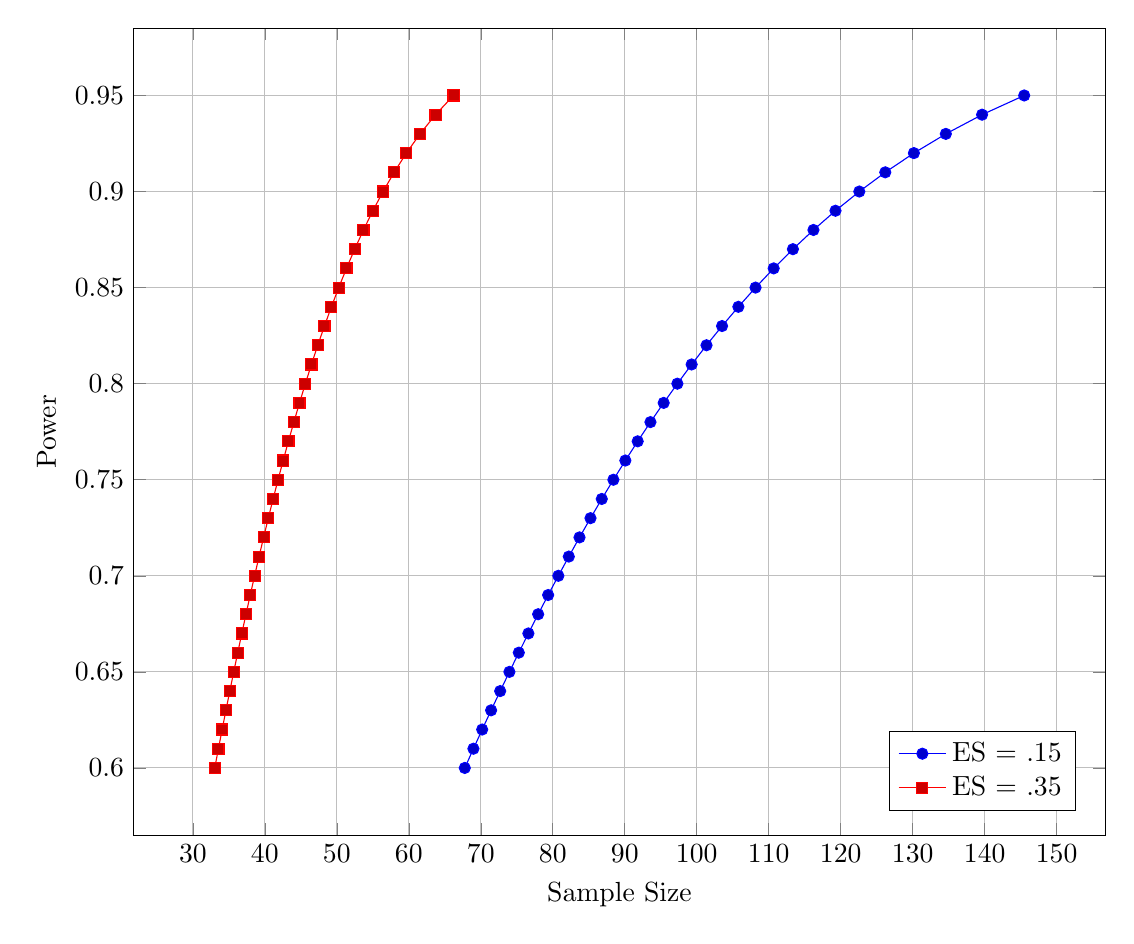
\begin{tikzpicture}
	\begin{axis}[grid=major,xlabel=Sample Size,ylabel=Power,scale=1.8, legend pos = south east]

\addplot coordinates {
(67.7774,	0.60)
(68.9775,	0.61)
(70.196,	0.62)
(71.4343,	0.63)
(72.6936	,0.64)
(73.9752,	0.65)
(75.2807,	0.66)
(76.6116,	0.67)
(77.9697,	0.68)
(79.3569,	0.69)
(80.7752,	0.70)
(82.2269,	0.71)
(83.7145,	0.72)
(85.2407,	0.73)
(86.8085	,0.74)
(88.4213,	0.75)
(90.0829	,0.76)
(91.7974,	0.77)
(93.5697	,0.78)
(95.4052,	0.79)
(97.31,	0.80)
(99.2912,	0.81)
(101.357,	0.82)
(103.517,	0.83)
(105.783,	0.84)
(108.167,	0.85)
(110.686,	0.86)
(113.36,	0.87)
(116.212,	0.88)
(119.273,	0.89)
(122.583	,0.90)
(126.19,	0.91)
(130.165	,0.92)
(134.602,	0.93)
(139.639,	0.94)
(145.49	,0.95)};
\addlegendentry{ES = .15}

\addplot coordinates{
(33.0406	,0.60)
(33.5515	,0.61)
(34.0702	,0.62)
(34.5975	,0.63)
(35.1338,	0.64)
(35.6797	,0.65)
(36.2358,	0.66)
(36.8028,	0.67)
(37.3815,	0.68)
(37.9727,	0.69)
(38.5772,	0.70)
(39.196,	0.71)
(39.8303,	0.72)
(40.481,	0.73)
(41.1496,	0.74)
(41.8375	,0.75)
(42.5462,	0.76)
(43.2777,	0.77)
(44.0338,	0.78)
(44.817,	0.79)
(45.6299,	0.80)
(46.4756,	0.81)
(47.3574,	0.82)
(48.2795,	0.83)
(49.2468,	0.84)
(50.265,	0.85)
(51.3408,	0.86)
(52.4828,	0.87)
(53.7013	,0.88)
(55.0092,	0.89)
(56.423	,0.90)
(57.9647	,0.91)
(59.6634,	0.92)
(61.5598,	0.93)
(63.7132,	0.94)
(66.2148,	0.95)};
\addlegendentry{ES = .35}

\end{axis}
\end{tikzpicture}
\caption[pH Power Graph]{pH Power Graph.  The power is shown as a function of pH}
\label{fig:pHPowerGraph}
\end{figure}%maybe transfer to table notation instead of coordinates
		\subsection{ANC and Nitrate}
			\begin{figure}[htbp]
\centering
\caption[A priori ANC and Nitrate Power Graph]{A priori ANC and Nitrate Power Graph.  The power graphs for ANC and Nitrate are the same because they both have the same number of predictors.}
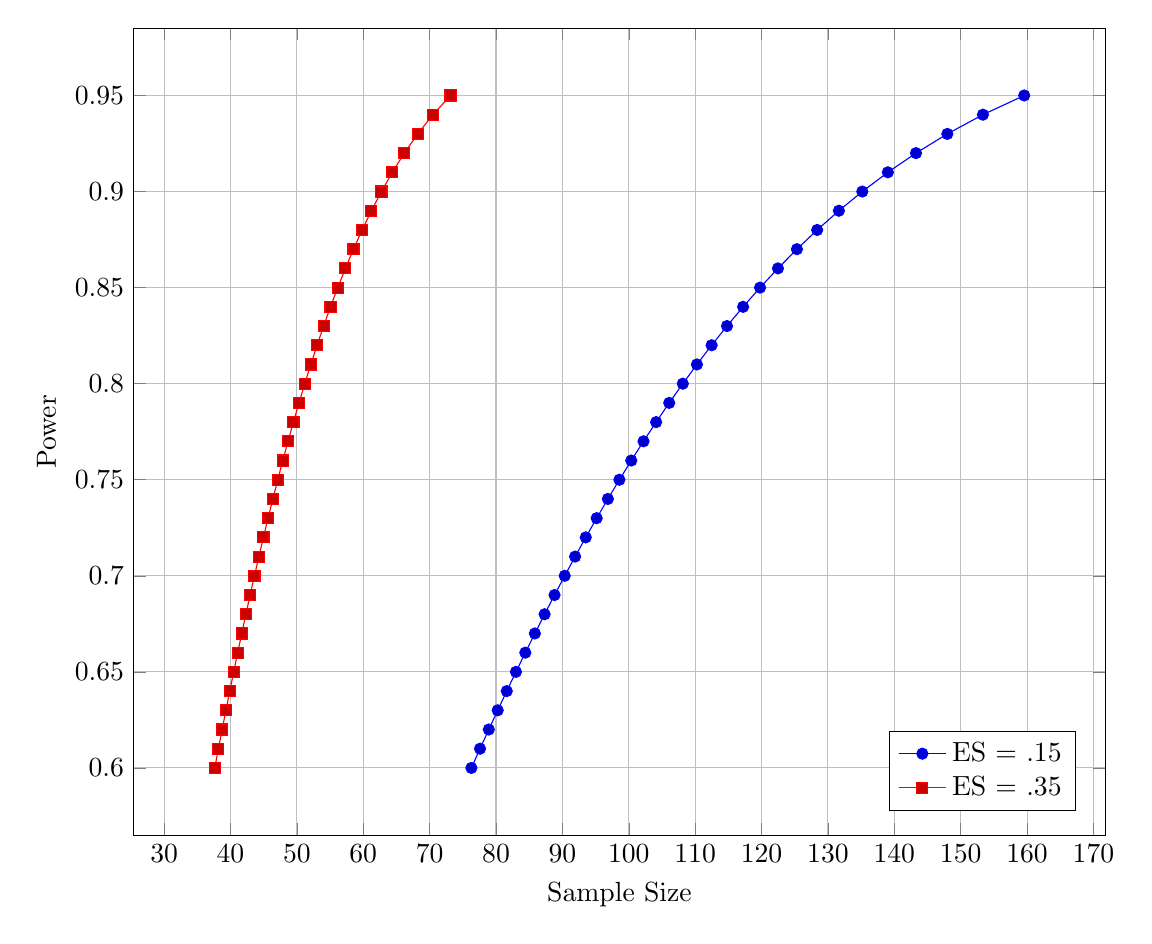
\begin{tikzpicture}
	\begin{axis}[grid=major,xlabel=Sample Size,ylabel=Power,scale=1.8, legend pos= south east] 
\addplot coordinates{
(76.2911	,0.60)
(77.592,	0.61)
(78.9124,	0.62)
(80.2534	,0.63)
(81.6164	,0.64)
(83.0029	,0.65)
(84.4146,	0.66)
(85.853	,0.67)
(87.32,	0.68)
(88.8177,	0.69)
(90.3482,	0.70)
(91.914,	0.71)
(93.5176,	0.72)
(95.162,	0.73)
(96.8504	,0.74)
(98.5864,	0.75)
(100.374,	0.76)
(102.218,	0.77)
(104.122,	0.78)
(106.094,0.79)
(108.139,	0.80)
(110.265,	0.81)
(112.48,	0.82)
(114.795,	0.83)
(117.222,	0.84)
(119.775	,0.85)
(122.471,	0.86)
(125.33,	0.87)
(128.378,	0.88)
(131.647,	0.89)
(135.179,	0.90)
(139.027,	0.91)
(143.263,	0.92)
(147.987,	0.93)
(153.347,	0.94)
(159.566,	0.95)};
\addlegendentry{ES = .15}

\addplot coordinates{
(37.6275,	0.60)
(38.1808,	0.61)
(38.7424,	0.62)
(39.3129,	0.63)
(39.8929,	0.64)
(40.4829,	0.65)
(41.0838,	0.66)
(41.6961,	0.67)
(42.3208,	0.68)
(42.9585,	0.69)
(43.6104,	0.70)
(44.2774,	0.71)
(44.9606,	0.72)
(45.6612,	0.73)
(46.3808,	0.74)
(47.1207,	0.75)
(47.8827,	0.76)
(48.6687,	0.77)
(49.4809,	0.78)
(50.3216,	0.79)
(51.1938,	0.80)
(52.1007,	0.81)
(53.0458,	0.82)
(54.0337,	0.83)
(55.0693,	0.84)
(56.1588,	0.85)
(57.3093,	0.86)
(58.5299,	0.87)
(59.8314,	0.88)
(61.2275	,0.89)
(62.7358,	0.90)
(64.3793,	0.91)
(66.1888,	0.92)
(68.2074,	0.93)
(70.4977,	0.94)
(73.1559,	0.95)};
\addlegendentry{ES = .35}

				
\end{axis}
\end{tikzpicture}
\label{fig:ANCnNPowerGraph}
\end{figure}
		\subsection{Sulfate}
			\begin{figure}[htbp]
\centering
\caption[A priori Sulfate Power Graph]{A priori Sulfate Power Graph}
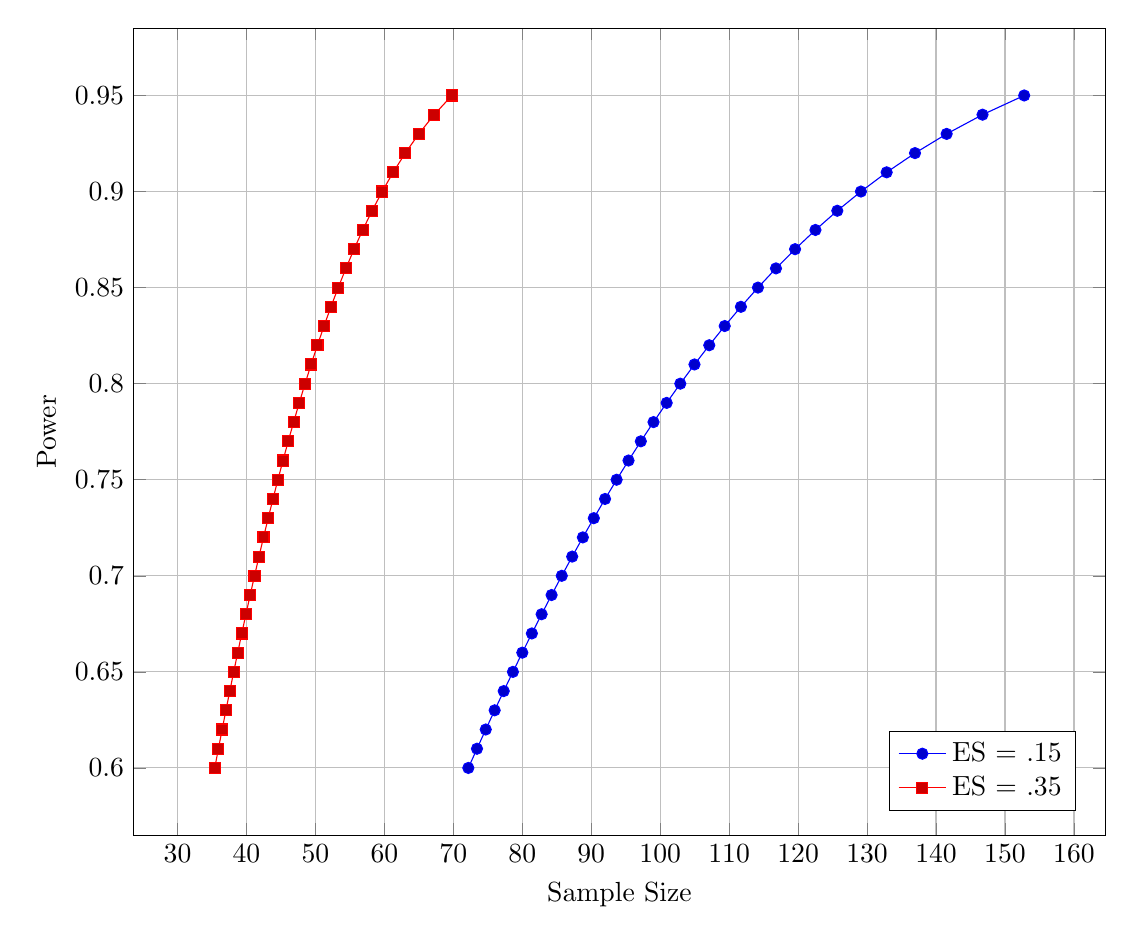
\begin{tikzpicture}
	\begin{axis}[grid=major,xlabel=Sample Size,ylabel=Power,scale=1.8, legend pos = south east] 
\addplot coordinates{
(72.1769,	0.60)
(73.4295,	0.61)
(74.701,	0.62)
(75.9928,	0.63)
(77.3061,	0.64)
(78.6423,	0.65)
(80.0031,	0.66)
(81.3899,	0.67)
(82.8048,	0.68)
(84.2495,	0.69)
(85.7262,	0.70)
(87.2373,	0.71)
(88.7853,	0.72)
(90.373,	0.73)
(92.0036,	0.74)
(93.6806,	0.75)
(95.4078,	0.76)
(97.1895,	0.77)
(99.0308,	0.78)
(100.937,	0.79)
(102.915,	0.80)
(104.971,	0.81)
(107.115,	0.82)
(109.356,	0.83)
(111.705,	0.84)
(114.177,	0.85)
(116.789,	0.86)
(119.559,	0.87)
(122.513,	0.88)
(125.683,	0.89)
(129.108,	0.90)
(132.84,	0.91)
(136.951,	0.92)
(141.538,	0.93)
(146.743,	0.94)
(152.786,	0.95)};
\addlegendentry{ES = .15}

\addplot coordinates{
(35.399	,0.60)
(35.932,	0.61)
(36.4731,	0.62)
(37.0229,	0.63)
(37.582,	0.64)
(38.1509,	0.65)
(38.7303,	0.66)
(39.321,	0.67)
(39.9236,	0.68)
(40.5391,	0.69)
(41.1683,	0.70)
(41.8122,	0.71)
(42.472,	0.72)
(43.1488,	0.73)
(43.8439,	0.74)
(44.5589,	0.75)
(45.2954,	0.76)
(46.0553,	0.77)
(46.8407,	0.78)
(47.6539,	0.79)
(48.4977,	0.80)
(49.3752,	0.81)
(50.29,	0.82)
(51.2464,	0.83)
(52.2493,	0.84)
(53.3046,	0.85)
(54.4195	,0.86)
(55.6024,	0.87)
(56.8641,	0.88)
(58.218,	0.89)
(59.6811,	0.90)
(61.2758,	0.91)
(63.0322,	0.92)
(64.9923,	0.93)
(67.2171,	0.94)
(69.8003,	0.95)};
\addlegendentry{ES = .35}


\end{axis}
\end{tikzpicture}
\label{fig:SulfatePowerGraph}
\end{figure}
		\subsection{Time Variables}
			\begin{figure}
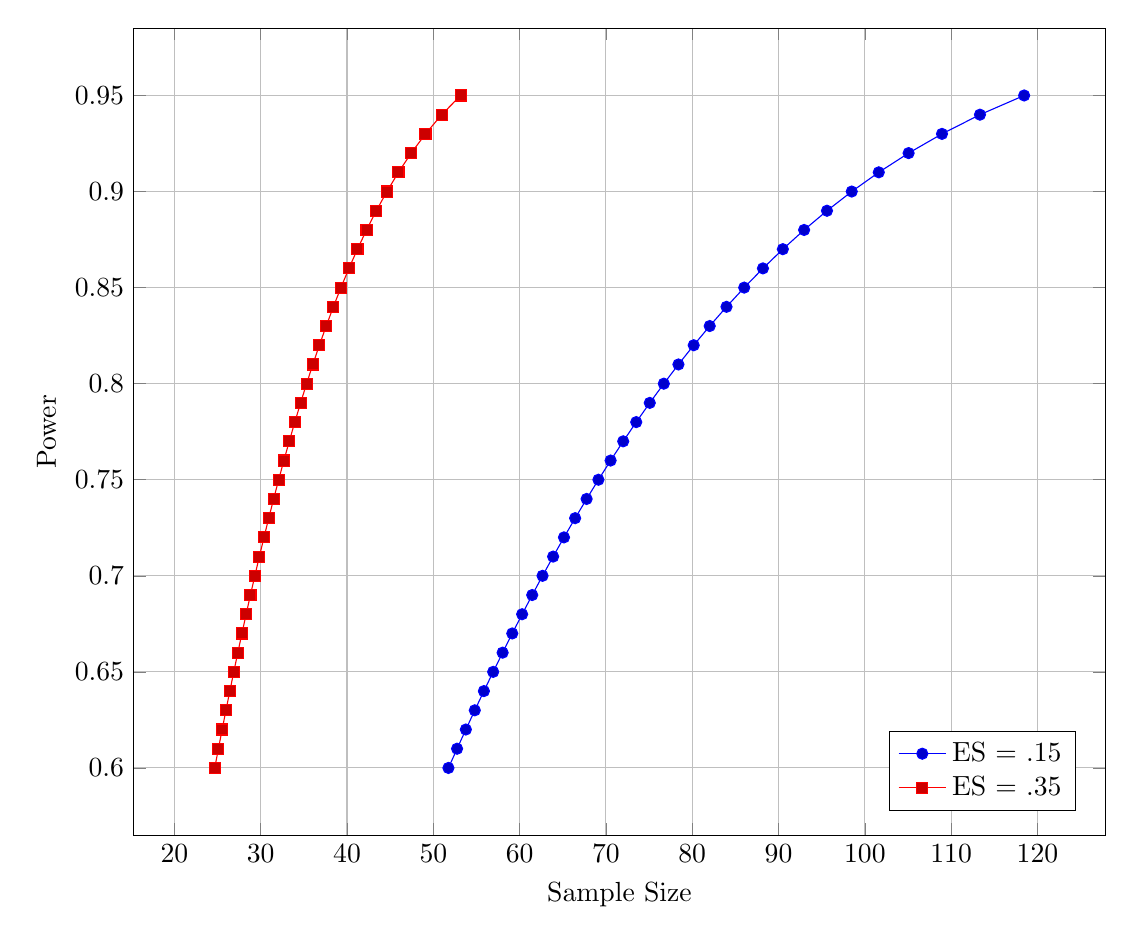
\begin{tikzpicture}
	\begin{axis}[grid=major,xlabel=Sample Size,ylabel=Power,scale=1.8, legend pos= south east] 
\addplot coordinates{
(51.7495	,0.60)
(52.7503,	0.61)
(53.7678,	0.62)
(54.8031,	0.63)
(55.8574,	0.64)
(56.9318,0.65)
(58.0275,	0.66)
(59.1461,	0.67)
(60.289,	0.68)
(61.4578,	0.69)
(62.6543,	0.70)
(63.8806,	0.71)
(65.1387,	0.72)
(66.4311,	0.73)
(67.7605,	0.74)
(69.1297,	0.75)
(70.5422,	0.76)
(72.0015,	0.77)
(73.512,	0.78)
(75.0783,	0.79)
(76.7058,	0.80)
(78.4009,	0.81)
(80.1708,	0.82)
(82.0239,	0.83)
(83.9701,	0.84)
(86.0213,	0.85)
(88.1917,	0.86)
(90.4986,	0.87)
(92.9634,	0.88)
(95.6129,	0.89)
(98.4816,	0.90)
(101.614,	0.91)
(105.072,	0.92)
(108.939,	0.93)
(113.339,	0.94)
(118.46	,0.95)};
\addlegendentry{ES = .15}

\addplot coordinates{
(24.6688	,0.60)
(25.095,	0.61)
(25.5284,	0.62)
(25.9694,	0.63)
(26.4186,	0.64)
(26.8765,	0.65)
(27.3435,	0.66)
(27.8203,	0.67)
(28.3075,	0.68)
(28.8059,	0.69)
(29.3161,	0.70)
(29.8392,	0.71)
(30.3758,	0.72)
(30.9272,	0.73)
(31.4944,	0.74)
(32.0787,	0.75)
(32.6815,	0.76)
(33.3044,	0.77)
(33.9492,	0.78)
(34.6179,	0.79)
(35.3129,	0.80)
(36.0368,	0.81)
(36.7927,	0.82)
(37.5842,	0.83)
(38.4156,	0.84)
(39.292,	0.85)
(40.2194,	0.86)
(41.2052,	0.87)
(42.2586,	0.88)
(43.3911,	0.89)
(44.6174,	0.90)
(45.9568,	0.91)
(47.4353,	0.92)
(49.089,	0.93)
(50.9706,	0.94)
(53.1614,	0.95)};
\addlegendentry{ES = .35}


\end{axis}
\end{tikzpicture}
\caption[Time Variables Power Graph]{Time Variables Power Graph}
\label{fig:TVPowerGraph}
\end{figure}



















